/home/glib/Annales/data/annales.sty
\versionCompil



\usepackage{booktabs}
\usepackage{pdfpages}
\usepackage{listings}
\usepackage{color}
 
\definecolor{codegreen}{rgb}{0,0.6,0}
\definecolor{codegray}{rgb}{0.5,0.5,0.5}
\definecolor{codepurple}{rgb}{0.58,0,0.82}
\definecolor{backcolour}{rgb}{0.95,0.95,0.92}
 
\lstset{
    escapeinside={\\}{}, 
    basicstyle=\tiny  
    backgroundcolor=\color{backcolour},   
    commentstyle=\color{codegreen},
    keywordstyle=\color{magenta},
    numberstyle=\tiny\color{codegray},
    stringstyle=\color{codepurple},
    basicstyle=\footnotesize\ttfamily,
    breakatwhitespace=false,         
    breaklines=true,                 
    captionpos=b,                    
    keepspaces=true,                 
    numbers=left,                    
    numbersep=5pt,                  
    showspaces=false,                
    showstringspaces=false,
    showtabs=false,                  
    tabsize=2
}


\DeclareRobustCommand{\rchi}{{\mathpalette\irchi\relax}}
\newcommand{\irchi}[2]{\raisebox{\depth}{$#1\chi$}}

\usepackage{pdfpages}
\usepackage{hyperref}
\usepackage[toc,page]{appendix} 

\newcommand{\poo}{{p_{0 0}}^{-s}}
\newcommand{\pii}{{p_{1 1}}^{-s}}
\newcommand{\poodeux}{{p_{0 0}}^{-2s}}
\newcommand{\piideux}{{p_{1 1}}^{-2s}}
\newcommand{\poi}{{p_{0 1}}^{-s}}
\newcommand{\pio}{{p_{1 0}}^{-s}}
\newcommand{\poiio}{{(p_{0 1}\,p_{1 0})}^{-s}}
\newcommand{\pooii}{{(p_{0 0}\,p_{1 1})}^{-s}}
\usepackage{caption}
\setlength{\parindent}{0pt}
\usepackage{float}
\usepackage{hyperref}
\hypersetup{
    colorlinks=true,
    linkcolor=blue,
    filecolor=magenta,      
    urlcolor=cyan,
}

\newtheorem{df}{Definition}
\newtheorem{definition}{Definition}
\newtheorem{nota}{Notation}
\newtheorem{rmk}{Remark}
\newtheorem{prop}{Property}

\usepackage{tikz}

\let\oldsection\section
\let\oldsubsection\subsection

\begin{document}
\begin{titlepage}
	
	\newcommand*{\Logos}{../latex-figures/presentation-figures}
	\newcommand{\HRule}{\rule{\linewidth}{0.5mm}}
	
	\center
	
	\textsc{\LARGE Ecole Normale Superieure de Lyon}\\[1.5cm]
	\textsc{\Large Computer Science Department}\\[0.5cm]
	\textsc{\large Master's Internship Report}\\[2cm]
	
	\HRule \\[0.4cm]
	{ \LARGE \bfseries Asymptotics on Lempel-Ziv'78 compression}\\[0.4cm]
	\HRule \\[2cm]
	
	\begin{minipage}{0.4\textwidth}
		\begin{flushleft} \large
			\emph{Intern:}\\
			Guillaume \textsc{Duboc}\\
		\end{flushleft}
	\end{minipage}
	~
	\begin{minipage}{0.4\textwidth}
		\begin{flushright} \large
			\emph{Supervisor:} \\
			Wojtek \textsc{Szpankowski}\\[0.5cm]
		\end{flushright}
	\end{minipage}\\[3cm]
	
	{\large Center for Science of Information - Purdue University}\\[0.5cm]
	{\large May 21st - August 8th, 2018}\\
	
	\begin{figure}[!b]
		\begin{minipage}[c]{.4\linewidth}
			\centering
			\includegraphics[height=1.9cm]{\Logos/ens.png}\\[1cm]
			�cole Normale Sup�rieure de Lyon
		\end{minipage} \hfill
		\begin{minipage}[c]{.4\linewidth}
			\centering
			\includegraphics[height=2.1cm,
								trim = 0 0.5cm 0 0.5cm,
								clip=true]{\Logos/logoCSOI.png}\\[1cm]
			Center for Science of Information
		\end{minipage}
	\end{figure}
	
	\vfill
	
\end{titlepage}


% \raggedbottom
\titre{Asymptotics on Lempel-Ziv 78 compression}
\abstract{Diving into universal data compression through the analysis of the
Lempel-Ziv78 algorithm - with the help of probabilistic models, computer simulation
and complex analysis.}

% Veuillez ne pas modifier ce titre SVP.
\tableofcontents

\section{ Introduction }

\emph{Data compression}, \emph{source coding}, or \emph{bit-rate reduction} involve encoding information using fewer bits than the original representation.

\subsection{ Introduction to the problem }

Data compression is achieved by different types of algorithms, but in order
to study it formally we use a formal definition of a data compression scheme. 
First, we describe an algorithm which operates on words - 
in our case, Lempel-Ziv 78.
Then, we introduce a probabilitic model representing
the data to be compressed, which allows us to quantify
the efficiency of the algorithm.


\subsubsection{ Compression algorithm : Lempel-Ziv 78 }

\begin{definition}
    A \emph{compression algorithm} is a pair of functions on
    words $(\mathcal{C}, \mathcal{D})$ - compressor and 
    decompressor.
\end{definition}

\begin{definition}
    \label{def:lossless}
    A \emph{lossless} compression algorithm decompresses 
    the exact same data that was compressed in the first place.
\end{definition}

\begin{rmk}
    We will not describe the decompression part of 
    our algorithms, considering that the possibility
    of decompression is obvious in the case of LZ78.
\end{rmk}

In general, Lempel-Ziv algorithms dictionary-based scheme
which exploit previously seen patterns and redundancy to 
save off coding space. 
The Lempel-Ziv'78 (LZ'78) that partitions a sequence into 
phrases or blocks of variable size such that a new phrase
is the shortest substring not seen in the past as a phrase. 
Every such phrase is encoded by the index of its prefix 
appended by a symbol; thus the LZ'78 code contains the 
pairs \verb|(pointer, symbol)|.
For example, the string 
\centers{11001010001000100} of length 17 is parsed
as 
\centers{(1)(10)(0)(101)(00)(01)(000)(100)}
which can be be 
encoded in the following digital search tree:

\centers{
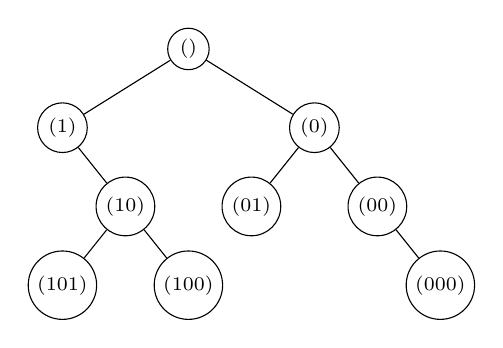
\begin{tikzpicture}[
    level 1/.style={level distance=10mm,sibling distance=32mm},
    level 2/.style={level distance=10mm,sibling distance=16mm},
    level 3/.style={level distance=10mm,sibling distance=16mm},
    font=\scriptsize,inner sep=2pt,every node/.style={draw,circle,minimum size=3ex}]
  ]
  \node {()}
    child {node {(1)}
        child[missing]
        child {node {(10)}
            child {node {(101)}}
            child {node {(100)}}
        }
    }
    child {node {(0)}
        child {node {(01)}}
        child {node {(00)}
            child[missing]
            child {node {(000)}}
        }
    }
        ;
\end{tikzpicture}
}




\subsubsection{ Probabilistic models }

\begin{df}
    \label{def:source}
    Let $\mathcal{A}$ be an alphabet.
    An \emph{information source} is a one-sided infinite sequence of random
    variables $(X_k)_{k=1}^{\pinf}$ with each $X_k$ 
    having values in $\mathcal{A}$.
\end{df}

\begin{rmk}
    \label{rmk:sequence}
    Each realization of an information source is called a 
    \emph{sequence} or \emph{word}.
\end{rmk}

\begin{rmk}
    \label{rmk:source}
    \emph{Defining} the law of the $X_k$ produces out different
    models for data generation which can be studied mathematically
    and \emph{simulated}.
\end{rmk}

\begin{df}
    \label{def:memoryless}
    A \emph{memoryless source} is an \emph{information source}
    for which the $X_k$ are mutually independent, following
    the uniform law on $\mathcal{A} = \{ a_1, \dots, a_V \}$ :
    \centers{$
        \proba{  X_k = a_k  } = p_k 
        \qquad \textmd{with } \,\Sum{i=1}{V} \,p_i = 1
    $}
\end{df}

\begin{rmk}
    \label{rmk:memoryless}
    This is the simplest information source and it has been 
    studied successfully in the past, but it is not a realistic 
    model. We replace it with the following Markov model whenever 
    possible.
\end{rmk}

\begin{df}
    \label{def:markov}
    A \emph{Markov source} is an \emph{information source}
    with a Markov dependency between successive symbols.
\end{df}

\begin{df}
    \label{def:markovorder}
    A \emph{Markov source of order $r$} is a Markov source
    for which each symbol apparition depends on the previous 
    $r$ symbols.
\end{df}

\begin{rmk}
    \label{rmk:markov2}
    We will study Markov sources of order 1 - where each
    symbol simply depends on the previous one. This is 
    general enough, as Markov sources of superior order
    can be simulated by expanding the alphabet and 
    using a Markov source of order 1.
\end{rmk}

\subsubsection{ Entropy }

    In this study, we consider only two information sources:
    the \emph{memoryless} and the \emph{Markov} source.
    For the Markov source, we consider that there exists a 
    \emph{stationary distribution}.

    \begin{df}
        \label{def:entropy}
        The \emph{entropy} of an information is the average
        rate at which information is produced by a probabilistic
        source of information.
    \end{df}

    \begin{prop}
        \label{prop:memorylessentropy}
        The entropy of a \emph{memoryless source} on 
        alphabet $\mathcal{A} = \{ a_1,\dots,a_V \}$ is:
        \centers{$ \Sum{i=1}{} p_i \log p_i$}
    \end{prop}

    \begin{prop}
        \label{prop:markoventropy}
        The entropy of a \emph{Markov source} with probability
        $(p_{i j})_{(i, j) \in { \{1,\dots,V\} }^2} $ and a 
        stationary distribution $(\pi_1, \dots, \pi_V)$ is:
        \centers{$ h = \Sum{i=1}{} \pi_i \Sum{j=1}{} p_{i j} \log p_{i j} $}
    \end{prop}

    
    The entropy gives a lower bound on the compression 
    ratio of lossless algorithms. Furthermore, in our
    case, for a memoryless or Markov source, the compression
    tends asymptotically to the entropy of the source:
    

    \begin{prop}
        \label{prop:lowerbound}
        \centers{$\underset{n\rightarrow\pinf}{\limt}\f{C_n}{n} = h$}
    \end{prop}


\subsubsection{ Probabilistic analysis }

Under this context, we can define and conduct a thorough
analysis of several random variables with different meanings
regarding the effectiveness of compression.

\begin{nota}
    \label{nota:universe}
    Let $n$ be an integer - the size of the considered words.
    Defining $\Omega_n$ the set of words of size $n$ on alphabet
    $\mathcal{A}$. Each word being an event, a natural probability
    space is given by considering the output of size $n$ of a Markov
    source.
\end{nota}

\begin{rmk}
    \label{rmk:probaspace}
    We will now study random variables defined 
    on this probability space. 
\end{rmk}

\begin{nota}
    \label{nota:output}
    $W_n$ denotes words of size $n$ output by a given Markov source.
\end{nota}

\begin{nota}
    \label{nota:numberphrases}
    The \emph{number of phrases} used to compress words of size $n$ ($W_n$) with
    LZ78 is given by $M_n(W_n)$ or simply $M_n$.
\end{nota}

\begin{rmk}
    \label{rmk:numberphrases}
    This is one of the most important variables to consider because,
    as it will appear shortly, it is closely tied to the \emph{compression 
    ratio} of LZ78.
\end{rmk}

\begin{df}
    \label{df:codelength}
    The \emph{codelength} is the \emph{number of bits} required 
    to encode the LZ78-compressed version of a word, denoted by $C(W_n)$ or $C_n$.
\end{df}

\begin{df}
    \label{df:compratio}
    The \emph{compression ratio} for words of size $n$ is the ratio between the 
    codelength and initial size of a word, $\f{C(W_n)}{|W_n|} = \f{C_n}{n}$.
\end{df}

\begin{rmk}
    \label{rmk:asymptotic}
    We focus now, as stated in the title of this report, on the asymptotical behavior - 
    for $n \rightarrow \pinf$ - of the compression ratio. Certainly this gives us 
    information about real-world compression, as files on our computer often attain
    large numbers when measured in bits. However, this assumption can be nuanced.
    For example, the speed of convergence towards this asymptotic behavior can make 
    a non-negligible difference in real-world application, as we will see later on
    when we talk about the difference between LZ'77 and LZ'78 and Optimal Parsing.
\end{rmk}



\subsection{ Theorems and Goals }

    There is a number of interrogations and results that surround
    the LZ'78 compression scheme, and that have been doing so for 
    some time now. These were proven for the simplistic memoryless
    source model which will allow us to formulate these as 
    theorems for memoryless sources. But the more interesting case
    of Markov sources has all these theorems become conjectures.
    My first job was to simulate the process and output visualizations
    that would disprove or make these results seem more likely.

    \begin{th}
        \label{th:clt}
        For memoryless source
    \end{th}


\section{ Numerical simulation of LZ78 for Markovian sources}
\renewcommand{\subsection}{\subsubsection}
\renewcommand{\section}{\oldsubsection}
\titre{Numerical simulations of LZ78 for Markovian sources}
% Veuillez ne pas modifier ce titre SVP.
% En cas de doute, pr�venez votre coordinateur.
% Compilez par: "latex main.tex".


\separation
\bk

% Quelques explications sur le sujet; articulation des parties; une page.



%%%%%%%%%%%%%%%%%%%%%%%%%%%%%%%%%%%%%%%%%%%%%%%%%%%%%%%%%%%%%%%%%%%%%%%%%%%%%%



\medskip

\section{Conditions of the experiment}
\subsection{Simulation details}

Simulations in this report follow this experimental
process :
	
\begin{itemize}

	\item Generating a random Markov chain of size 2 of matrix
 \centers{ $\begin{matrice}
			p_{0 0} & p_{0 1} \\
			p_{1 0} & p_{1 1} \\
		  \end{matrice}$}	 
 \item
 Generating $n_{\text{exp}} \sim 10^3$ words of length $n $ (or $n_{\text{word}}$), with $n \leq 10^6 - 10^7$
 
 \item Applying LZ78 on each of these words to estimate, for each $n$,
 the number of phrases $M_n$. A simple histogram of these values
 can be seen in figure 1.
 
 \item From this sampling of the random variable $M_n$ and other parameters such as the entropy of the Markov chain, computing
 
 	\begin{itemize}
 		\item the empirical mean ($\mu$) and the empirical variance ($\sigma^2$)
 		\item different theoretical expressions of the mean and variance
 	\end{itemize}
 	
 \item Using these expressions to standardize $M_n$ in different ways, plotting
 
 	\begin{itemize}
 		\item the probability distribution of $M_n$ (standardized)
 			  
 		\item the cumulative distribution function of $M_n$ (standardized)
 	\end{itemize}
 
 \item Finally, comparing the different theoretical expressions for the mean and 
 variance by plotting their differences for a large range of values of $n$, and
 a constant number of experiments $n_{\text{exp}}$.
\end{itemize}
 
%  \subsection{Example histogram}
%  This histogram represents the counts of the different 
%  values taken by $M_n$ for $n=10^6$. 
%  Each tick on the x-axis is a data point.
 
%  \centers{
%   \begin{minipage}{7cm}
   
    		
%         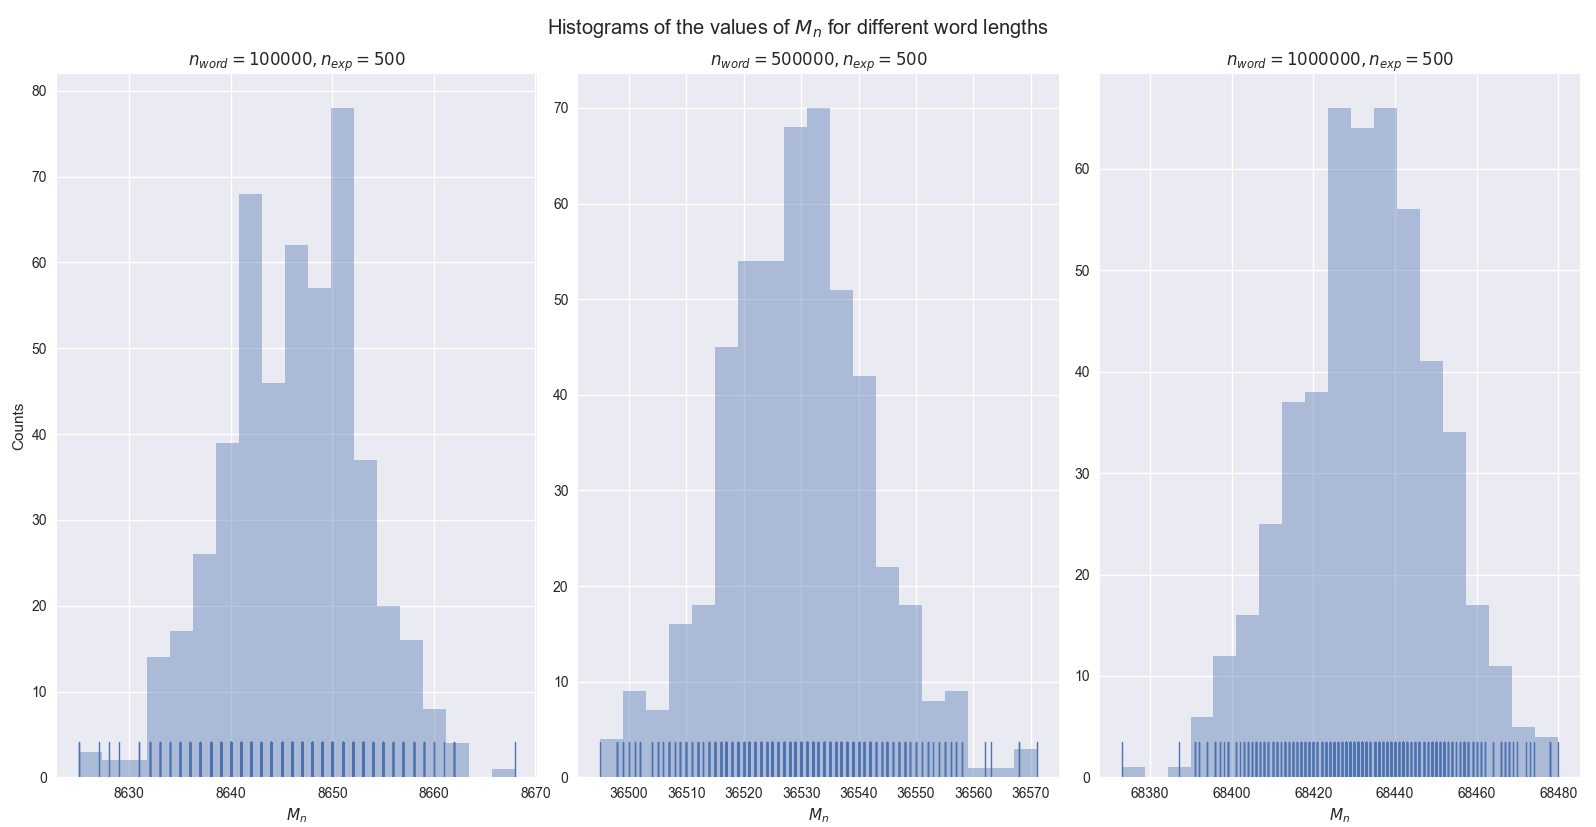
\includegraphics[width = 7cm,
%         				    trim = 27cm 0 0 0,
%         				    	clip=true]{M_n_raw_10e6_500.png}	
       
    
% 	\end{minipage}
% }

	\subsection{Empirical normalization}
 Using the empirical mean ($\mu$) and variance ($\sigma^2$) of the dataset to normalize $M_n$,
 this is a plot of the normalized distribution, compared to the normal distribution 
 in red :
 \centers{
  \begin{minipage}{6cm}
        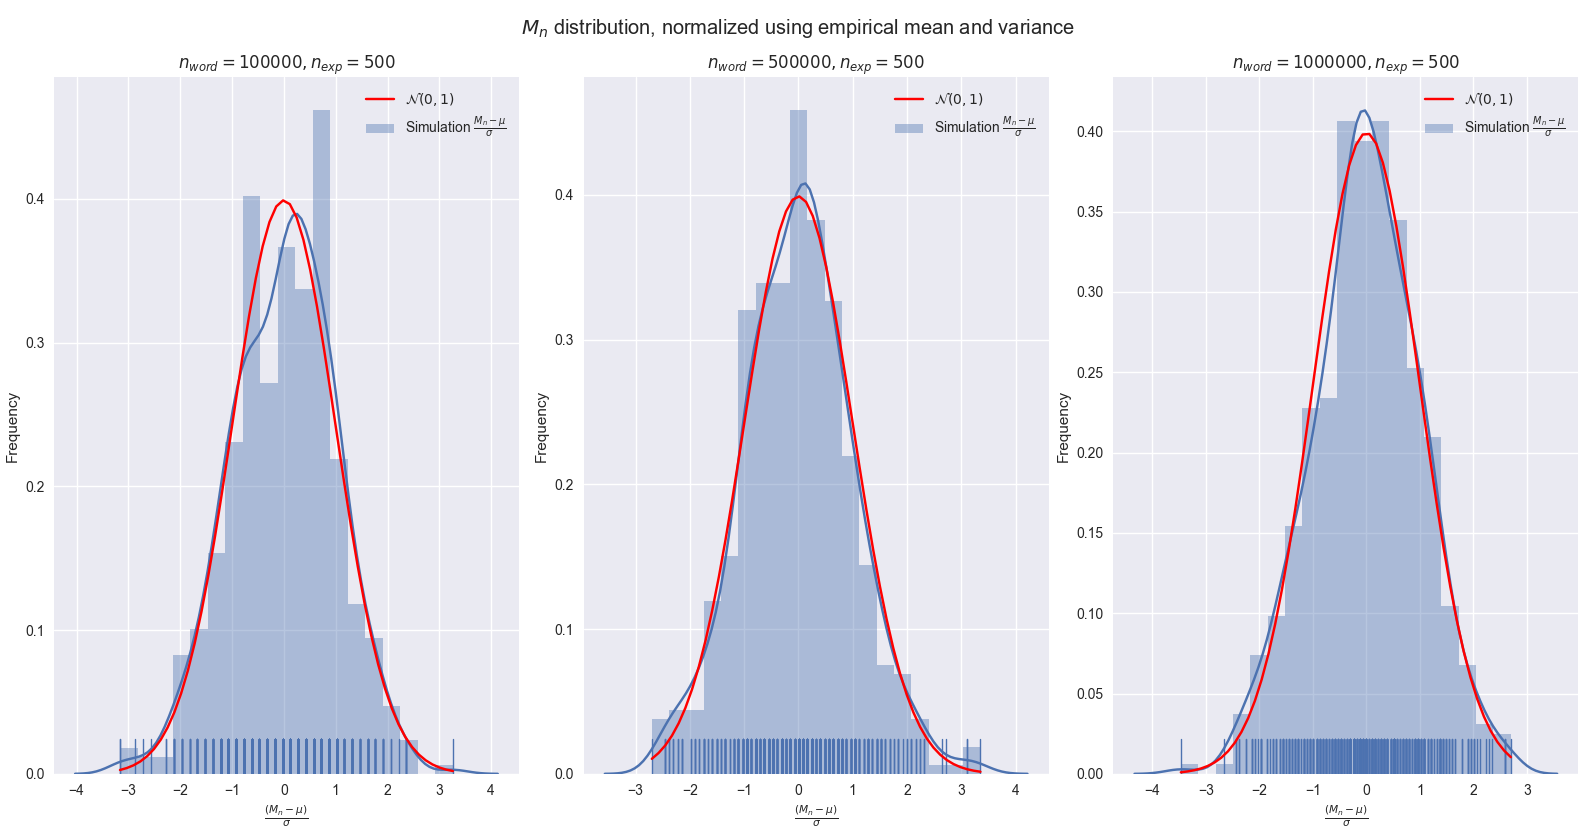
\includegraphics[width = 6cm,
        				    trim = 26.7cm 0 0 30,
        				    	clip=true]{empirical_normalization_10e6_500.png}	
	\end{minipage} 
}
	\noindent
	 and its cumulative distribution function in green, compared to the normal one in red:
 	\centers{
 	 \begin{minipage}{7cm}
        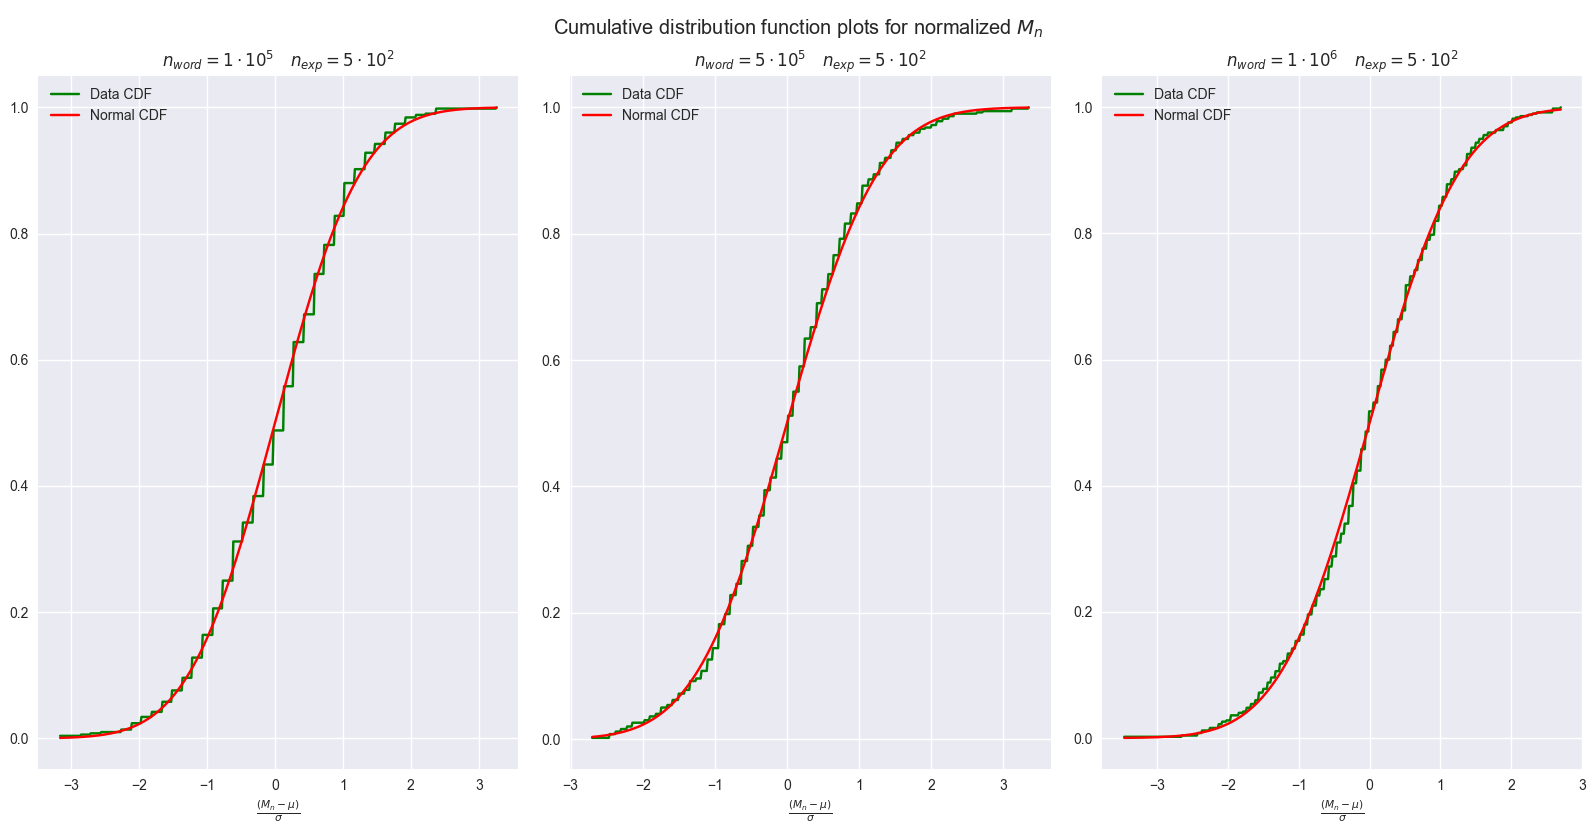
\includegraphics[width = 7cm,
        				    trim = 27cm 0 0 32,
        				    	clip=true]{cdf_1e6_500.png}
	\end{minipage} 
	}
	
	These simulations and figures strongly indicate that the general distribution
	of $M_n$ respects the central limit theorem. We now experiment with
	candidates for the variance of $M_n$ : $V_n$

	% In comments, because not really interesting
	% \centers{\question{Theoretical mean}}
	% I also tried to normalize $M_n$ using theoretical expressions
	% of the mean and variance. For the mean, the first order expression
	
	% \centers{$E_n \sim \f{nh}{\log_2(n)}$}
	
	% \noindent
	% is, under $n\leq 10^6$, not sufficient to center the distribution. I conducted a numerical analysis
	% of the difference between this expression and the empirical mean for growing 
	% values of $n$. In particular, here is how their difference, in black, compares with
	% different approximation functions 
	
	% \centers{
 	%  \begin{minipage}{9cm}
    %     \includegraphics[width = 9cm,
    %     				    trim = 14cm 0 13cm 20,
    %     				    	clip=true]{mean_analysis_2e4_500.png}	
	% \end{minipage} 
	% }
	
	% \noindent
	% This is not troubling as it was already predicted in the formula:
	
	% \centers{$E_n = 	\f{nh}{\log_2(n)} + \mathcal{O} \pa{ \f{n}{\log_2(n)} }$}
	
	% \pagebreak
	\section{Validating variance candidates}
	\subsection{A first expression}
	As it will be used in the next section, this is the detail of the expression

		\centers{ $\f{H^3 \sigma^2}{n \log_2^2 (n)}$ }
		
	from K. Lecket, N. Wormald and R. Neininger's paper 
	\textit{Probabilistic Analysis of Lempel-Ziv Parsing for Markov Sources},  :
		
	\centers{$\sigma^2 = \sigma_0^2 + \sigma_1^2$}
	\leftcenters{where}{$\sigma_i^2 = \f{\pi_i p_{i 0} p_{i 1}}{ H^3 } \pa { \log_2 \pa{ \f{ p_{i 0} }{ p_{i 1} } }
										+ \f{H_1 - H_0}{p_{0 1} + p_{1 0}} }^2$}
	\leftcenters{with}{$\pi_0 = \f{p_{1 0}}{p_{1 0} + p_{0 1}} \qquad \pi_1 = \f{p_{0 1}}{p_{1 0} + p_{0 1}}$}
	\leftcenters{and}{$H_i = -p_{i 0} \log_2(p_{i 0}) - p_{i 1} \log_2(p_{i 1}) \qquad H = \pi_0 H_0 + \pi_1 H_1 $}
	
	% \begin{remarque}
	% \noindent 
	% The first term in the squared part of $\sigma_i^2$ accounts for the expression of the variance for memoryless sources:
	
	% \begin{egalites}
	% & \ p_{i 0}\,p_{i 1} \log_2^2 \pa{ \f{p_{i 0} }{ p_{i 1} }}
	% 	& p_{i 0} \log_2^2(p_{i 0}) + p_{i 1} \log_2^2(p_{i 1}) 
	% 		- (- p_{i 0} \log_2(p_{i 0})  - p_{i 1} \log_2(p_{i 1}))^2 \\
	% 	&& h_2 - h^2
	% \end{egalites}
	
	% \end{remarque}	
	
	% \noindent
	% It seems, from simulations, that this variance is too small and doesn't
	% catch up with the empirical variance. Here is how they compare when plotted
	% together :
	
	% \centers{
 	%  \begin{minipage}{11cm}
    %     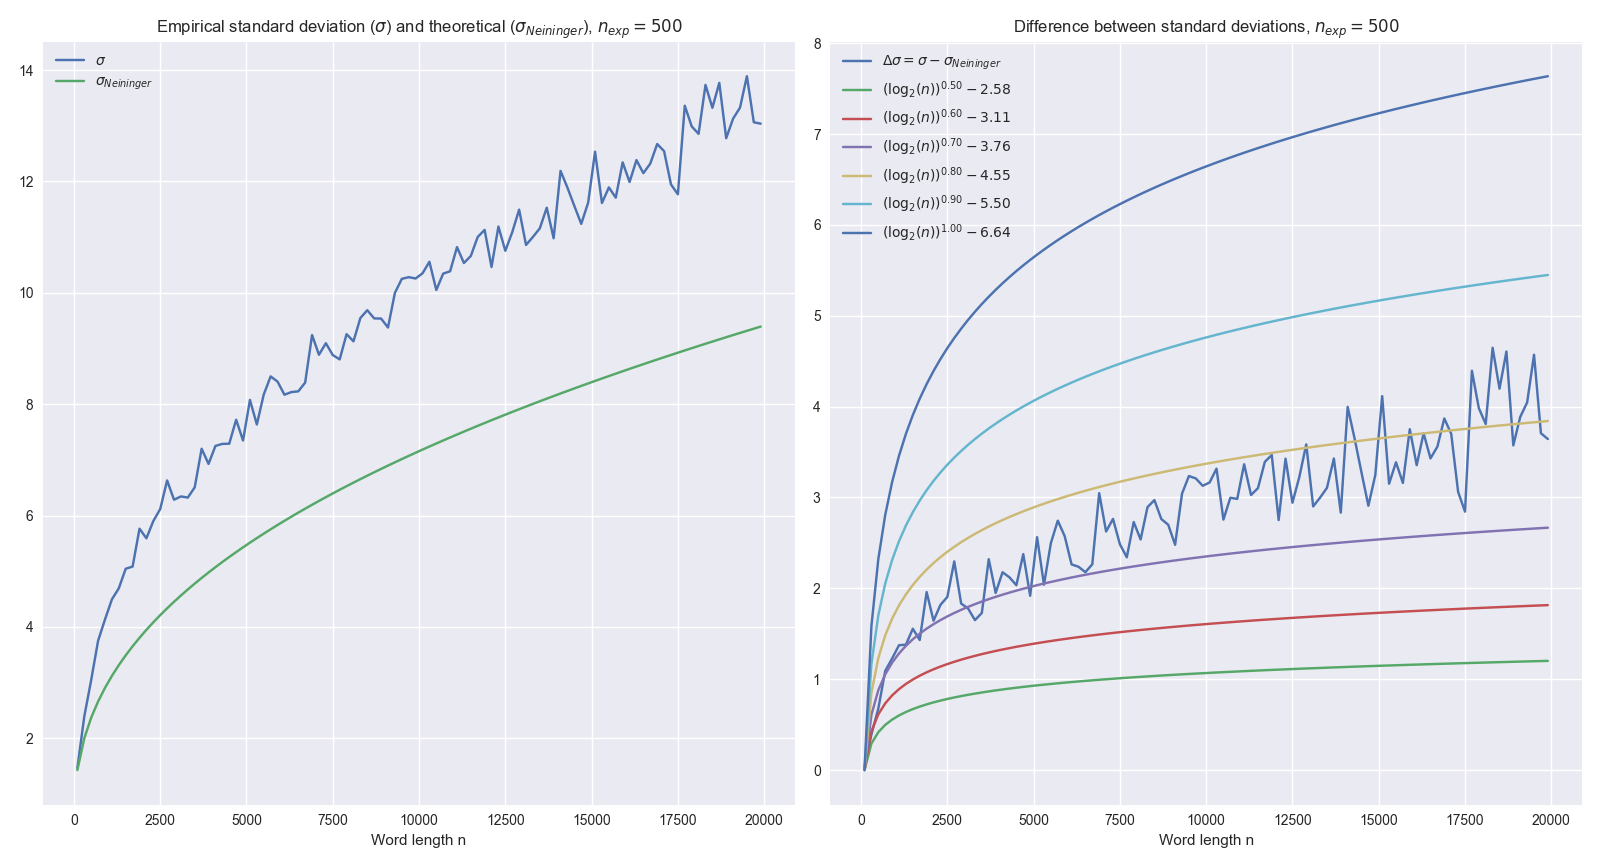
\includegraphics[width = 11cm,
    %     				    trim = 15 0 20cm 0,
    %     				    	clip=true]{std_analysis_2e4_500.png}	
	% \end{minipage} 
	% }
	
	% \pagebreak
	% \noindent
	% It seems, at first glance, that the increase would asymptotically be 
	% simply logarithmic
	
	% \centers{
 	%  \begin{minipage}{12cm}
    %     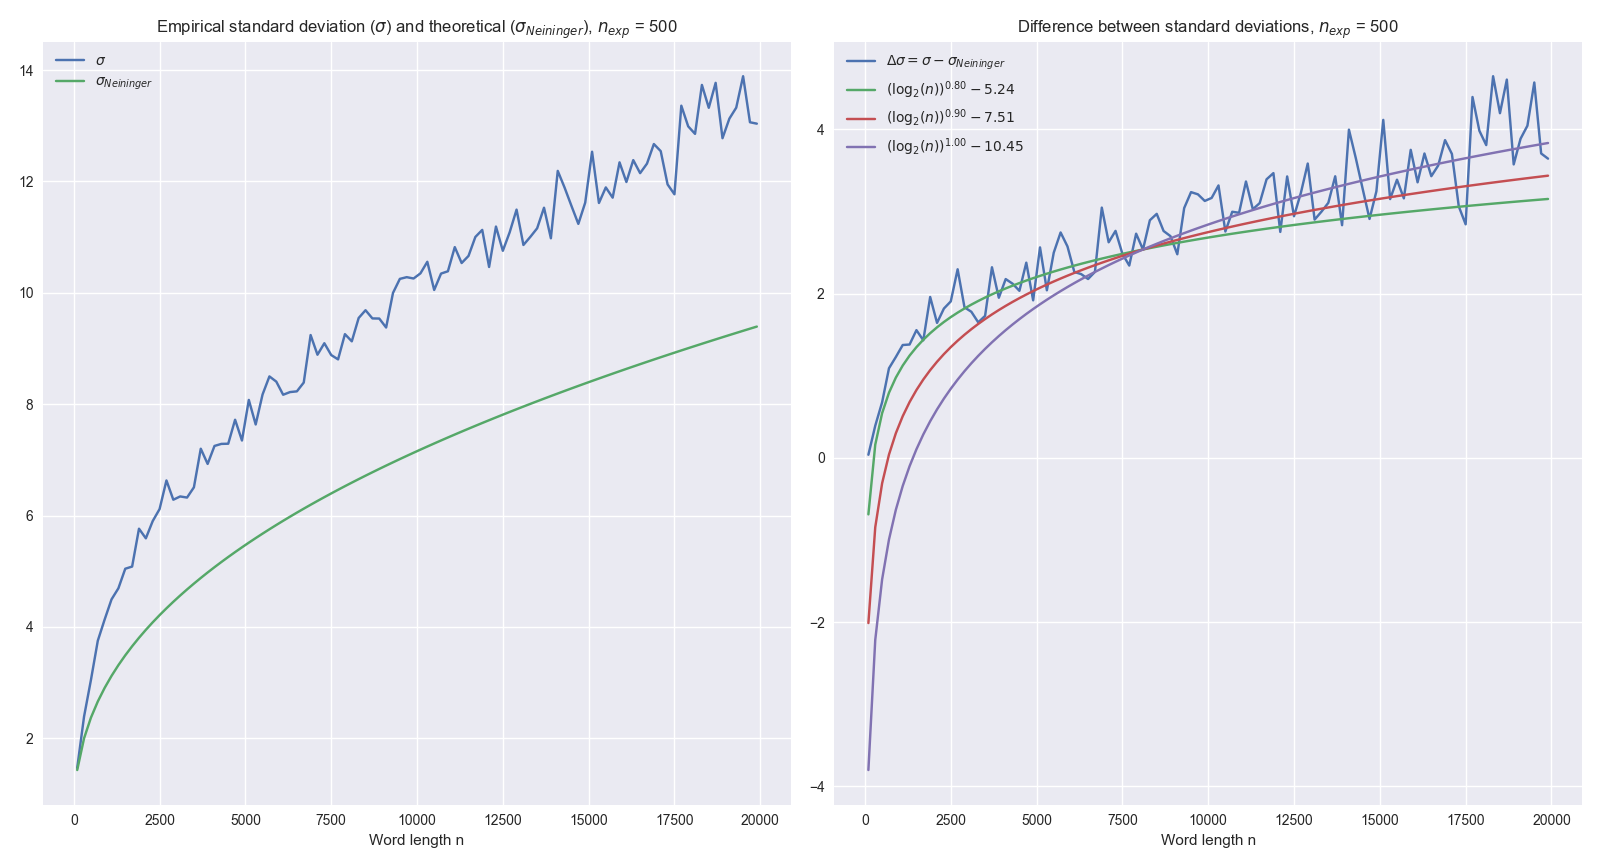
\includegraphics[width = 12cm,
    %     				    trim = 20.5cm 0 0 0,
    %     				    	clip=true]{std_analysis_approx_2e4_500.png}	
	% \end{minipage} 
	% }
	
	% \noindent 
	
	
% % Now, I'm trying to compute the variance using the formula from	Jacquet and Szpankowski, 
	\textit{Average profile of the Lempel-Ziv parsing scheme for a markovian source},
	using the formula for the variance $V_n$ :
	
	\centers{$V_n = \f{1}{h^3} \pa{
                -\f{\beta}{\omega} 
                -\f2{\omega} \pi \dot{Q}^{\star} \psi 
                -h^2 } \log(m) $}
	
This formula is obtained in the Markov independent model, so
$m$ is the number of sequences with which
we build a DST. Therefore, in my case, I would take

\centers{$ m \sim \f{n h}{\log(n)} $}

I computed the other terms from the general case as follows : 

	\begin{egalites}
	Since 
		& Q(s) & \begin{matrice}
							1 - {p_{0 0}}^{-s} & -{p_{0 1}}^{-s}  \\
							-{p_{1 1}}^{-s} & 1 - {p_{1 1}}^{-s}  \\
						  \end{matrice} \\[5mm]
	then
		& Q'(s) & \begin{matrice}
							\ln(p_{0 0}) {p_{0 0}}^{-s} & \ln(p_{0 1}) {p_{0 1}}^{-s}  \\
							\ln(p_{1 0}) {p_{1 1}}^{-s} & \ln(p_{1 1}) {p_{1 1}}^{-s}  \\
						  \end{matrice} \\[5mm]
	and
		& Q''(s) & \begin{matrice}
							-\ln^2(p_{0 0}) {p_{0 0}}^{-s} & -\ln^2(p_{0 1}) {p_{0 1}}^{-s}  \\
							-\ln^2(p_{1 0}) {p_{1 1}}^{-s} & -\ln^2(p_{1 1}) {p_{1 1}}^{-s}  \\
						  \end{matrice} \\[5mm]
	hence 
		& \det Q''(s)
			&  {(p_{0 0}\, p_{1 1})}^{-s} \ln^2 p_{0 0} \cdot \ln^2 p_{1 1}
				- {(p_{0 1}\, p_{1 0})}^{-s} \ln^2 p_{0 1} \cdot \ln^2 p_{1 0} \\
	\end{egalites}

	\leftencadre
		{therefore}
		{$ \beta = \rest{\pac{\det Q''(s)}}{s=-1} = p_{0 0}\, p_{1 1} \ln^2 p_{0 0} \cdot \ln^2 p_{1 1}
				- p_{0 1}\, p_{1 0} \ln^2 p_{0 1} \cdot \ln^2 p_{1 0} $}

	\begin{egalites}
	After that, with
		& {Q^\star}(s) & \begin{matrice}
							1 - {p_{1 1}}^{-s} & {p_{0 1}}^{-s}  \\
							{p_{1 0}}^{-s} & 1 - {p_{0 0}}^{-s}  \\
						  \end{matrice} \\[5mm]
	which gives
		& {\dot{Q}^\star}(s) & \begin{matrice}
							\ln(p_{1 1}) {p_{1 1}}^{-s} & - \ln(p_{0 1}) {p_{0 1}}^{-s}  \\
							- \ln(p_{1 0}) {p_{1 0}}^{-s} & \ln(p_{0 0}) {p_{0 0}}^{-s}  \\
						  \end{matrice}
	\end{egalites}

	\leftencadre
		{then}
		{$ \pi \dot{Q}^{\star} \psi =
			\pi_0 \, p_{1 1} \, \ln (p_{1 1}) 
			- \pi_1 \, p_{1 0} \ln (p_{1 0})
			- \pi_0\, p_{0 1} \ln (p_{0 1}) \\
			 	  + \pi_1 \, p_{0 0} \ln (p_{0 0})$}

	Finally since $Q^\star = \omega \Pi$
with $\Pi = \begin{matrice} \pi_0 & \pi_1 \\
							\pi_0 & \pi_1 
			\end{matrice}$, then in particular 
			
	\centers{$1 - p_{0 0} = q_{0 0}^\star = \omega \pi_0 = \omega \f{ p_{1 0}}{p_{1 0} + p_{0 1}}$}

    \leftencadre
		{so}
		{$ \omega = \f{ (p_{0 1} + p_{1 0}) \, (1 - p_{1 1})}
						  { p_{1 0} } = p_{0 1} + p_{1 0} $}


\begin{tabular}{lrrrrrrrr}
\toprule
{} &  2o/pqpsi &         V\_n &  beta/omega &       h\textasciicircum2 &  h\textasciicircum3 values &      logs &    omegas &        unhs \\
\midrule
0 &           -0.096184 &   17.562029 &   -0.623749 &  0.220193 &    0.103325 &  3.631080 &  0.802159 &    9.678203 \\
1 &            0.489107 &    4.683284 &   -0.868024 &  0.234073 &    0.113247 &  3.661644 &  0.434225 &    8.830250 \\
2 &           -0.496605 &  747.846171 &   -0.388158 &  0.019911 &    0.002810 &  2.429464 &  0.831697 &  355.926183 \\
3 &            0.001069 &    0.926064 &   -0.501488 &  0.433778 &    0.285694 &  3.970094 &  0.997360 &    3.500248 \\
4 &            0.934518 &   -6.943693 &   -0.965841 &  0.167062 &    0.068283 &  3.493010 &  0.294606 &   14.644827 \\
5 &           -0.039947 &    3.287372 &   -0.434456 &  0.319125 &    0.180277 &  3.816619 &  1.407304 &    5.547010 \\
6 &            0.044734 &   -0.079016 &   -0.513799 &  0.475516 &    0.327905 &  4.016028 &  0.931207 &    3.049666 \\
7 &            0.088811 &   -0.104380 &   -0.547647 &  0.467153 &    0.319292 &  4.007156 &  0.871306 &    3.131927 \\
8 &            0.169804 &    1.038286 &   -0.474413 &  0.266313 &    0.137432 &  3.726165 &  1.250839 &    7.276301 \\
9 &           -0.253274 &   68.726370 &   -0.569139 &  0.105030 &    0.034039 &  3.260952 &  0.837022 &   29.378420 \\
\bottomrule
\end{tabular}




\subsection{Using the Frobenius eigenvalue of $P(s)$}

\noindent
An expression which seems to be succesful for the variance is :

\centers{$ V_n =  \left( \ddot{\lambda}(-1) - { \dot{\lambda}(-1) }^2 \right) \f{n}{\ln^2 n} $}

\noindent Let's compute $\ddot{\lambda}(-1)$ with a Markov chain of order 1.

\leftcenters
    {In the paper,}
    {$ \ddot{\lambda}(-1) = \pi \ddot{P}(-1)\psi
                        + 2 \dot{\pi}(-1) \dot{P}(-1) \psi
                        - 2 \dot{\lambda}(-1) \dot{\pi}(-1) \psi $}
\noindent However, the relations defining $\pi(s)$ : 
   
        \centers{ $ \left\{
            \begin{array}{rl} \pi(s) P(s)  &= \lambda(s) \pi(s) \\
                          P(s) \psi(s) &= \lambda(s) \psi(s) \\
                          \pi(s) \psi(s) &= \lambda(s) 
            \end{array}
                    \right. $}
         
did not seem to allow me to directly compute $\dot{\pi}(s)$ (it seemed like I need
one more).
Therefore, I computed $\lambda(s)$ as the greatest 
eigenvalue of $P(s)$. Let $\chi$ the characteristic polynomial of $P(s)$,
and $\Delta$ its discrimant

\centers{$ \chi = (X - {p_{0 0}}^{-s}) 
                  (X - {p_{1 1}}^{-s}) 
                    - (p_{0 1} \, p_{1 0})^{-s} $}

\begin{egalites}
 and   & \Delta 
        & (\poo + \pii)^2 - 4[\pooii - \poiio] \\[2mm]
        && {p_{0 0}}^{-2s} 
                + {p_{1 1}}^{-s} - 2\pooii + 4\poiio
\end{egalites}

 Informally, we have this expression for $\lambda(s)$ 
where we need to decide which sign is the correct one :
\encadre{$ \lambda(s) = \f{ \poo + \pii \pm \sqrt{\Delta(s)}}{2} $}

\leftcenters
    {Since}
    {$\Delta(-1) 
        = (p_{0 0} + p_{1 1})^2 
                        - 2 p_{0 0} p_{1 1} 
                        + 4 p_{0 1} p_{1 0}
        = (p_{0 0} + p_{1 1} - 2)^2 $}
then $ \sqrt{ \Delta(-1) } = 2 - p_{0 0} - p_{1 1} = p_{0 1} + p_{1 0}$. 
Thus, picking the $+$ sign in the former expression, we verify that  
\centers{$ \lambda(-1) =  \f{ p_{0 0} + p_{1 1} + \sqrt{ \Delta(-1) } }
                                               {2} = 1 $}

\leftcenters
    {Derivating}
    {$ \dot{\lambda}(s) = \f12 \left( -\ln p_{0 0}\, \poo - \ln p_{1 1}\, \pii + \f{ \Delta'(s) }{ 2 \sqrt{\Delta(s)} } \right) $}

and the expression for $\Delta'(s)$
\centers{$ \Delta'(s) = - 2 \ln p_{0 0}\, \poodeux - 2 \ln p_{1 1}\, \piideux
                        + 2 \ln (p_{0 0} p_{1 1})\, \pooii 
                        - 4 \ln (p_{0 1} p_{1 0})\, \poiio $}
gives
\centers{$ \Delta'(-1) = - 2 \ln p_{0 0}\, {p_{0 0}}^2 - 2 \ln p_{1 1}\, {p_{1 1}}^2
                        + 2 \ln (p_{0 0} p_{1 1})\, (p_{0 0} p_{1 1})
                        - 4 \ln (p_{0 1} p_{1 0})\, (p_{0 1} p_{1 0})  $}

allowing to compute $\dot{\lambda}(-1)$. 
Numerically, we verified that $ \dot{\lambda}(-1) = h $. Derivating again yields

\centers{$ \ddot{\lambda}(s) =
                \f12 \left( \ln^2 p_{0 0} \poo + \ln^2 p_{1 1} \pii
                    + \f{ \Delta''(s) \sqrt{\Delta(s)} - \Delta'(s) \cdot \tf{\Delta'(s)}
                                                                            {2\sqrt{\Delta(s)}} }
                        {2\Delta(s)} \right)
                   $}

\leftcenters
    {with}
    {$ \Delta''(s) = 4 \ln^2 p_{0 0}\, \poodeux + 4 \ln^2 p_{1 1}\, \piideux
                     - 2 \ln^2 (p_{0 0} p_{1 1})\, \pooii
                     + 4 \ln^2 (p_{0 1} p_{1 0})\, \poiio $}

\leftencadre
    {Finally}
    {$\ddot{\lambda}(-1) = \f12 \left( \ln^2 p_{0 0}\, p_{0 0} + \ln^2 p_{1 1}\, p_{1 1}
                                + \f{ \Delta''(-1) \sqrt{\Delta(-1)} - \tf { {\Delta'(-1)}^2 }
                                                                              {2\sqrt{\Delta(-1)}} }
                                        {2\Delta(-1)} \right)
                         $}

The simulations using this coefficient for the variance are quite good. It also seems that 
this formula for the variance is equivalent to the one used in the unpublished paper 
\emph{Probabilistic Analysis of Lempel-Ziv Parsing for Markov Sources} by Leckey, 
Wormald and Neininger, but our two ways of deriving it differs. Numerical instability
might account for the tiny differences found for high $n$ values ($10^7$), although
this hasn't been verified. 
The code that computes it can be found in appendix \ref{app:comp_lam2},
and the rest of the code, with detailed procedures for reproducibility,
is hosted on GitHub in a repository that, for the moment, private.
Another way of computing $\lambda(s)$ is in appendix \ref{app:comp_lam1}. 

\centers{
 	 \begin{minipage}{11cm}
        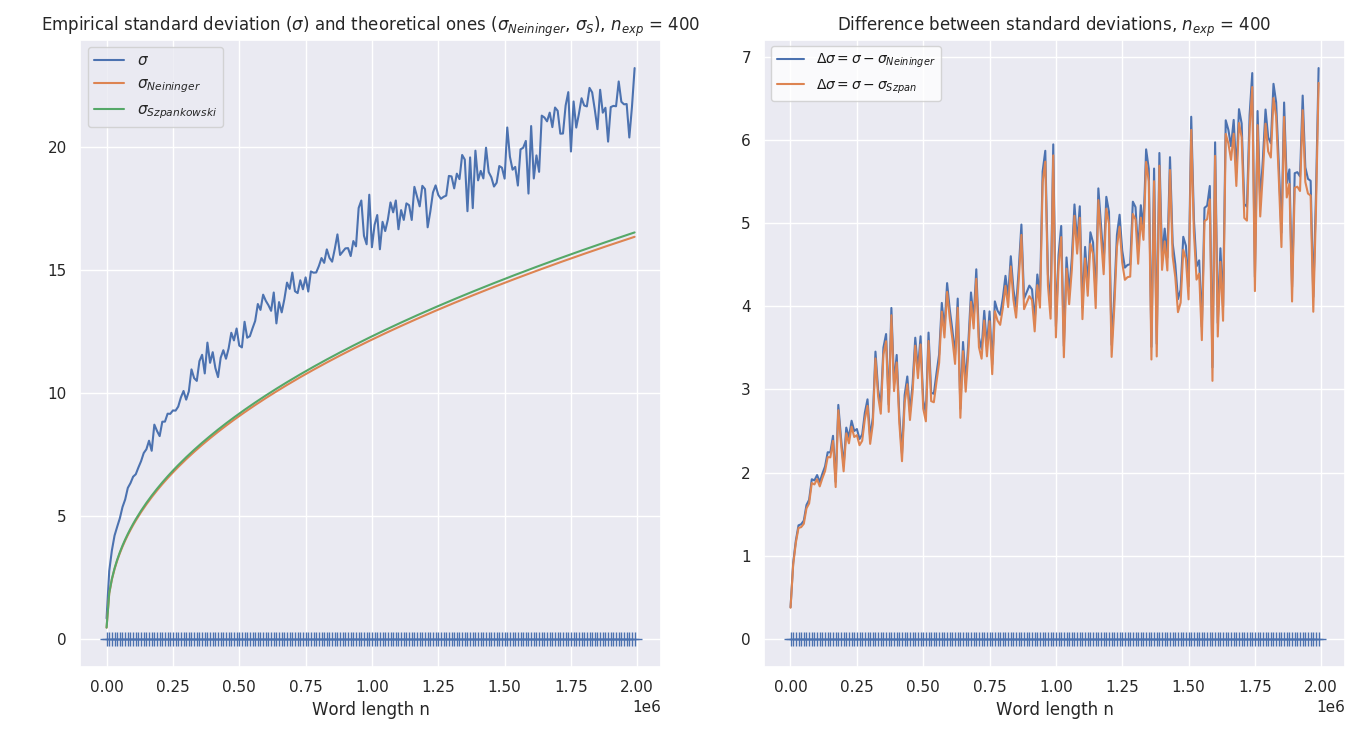
\includegraphics[width = 11cm,
        				    trim = 0 0 16.5cm 0,
        				    	clip=true]{./figs/eig_fig1.png}	
	\end{minipage} 
	}

\centers{
 	 \begin{minipage}{11cm}
        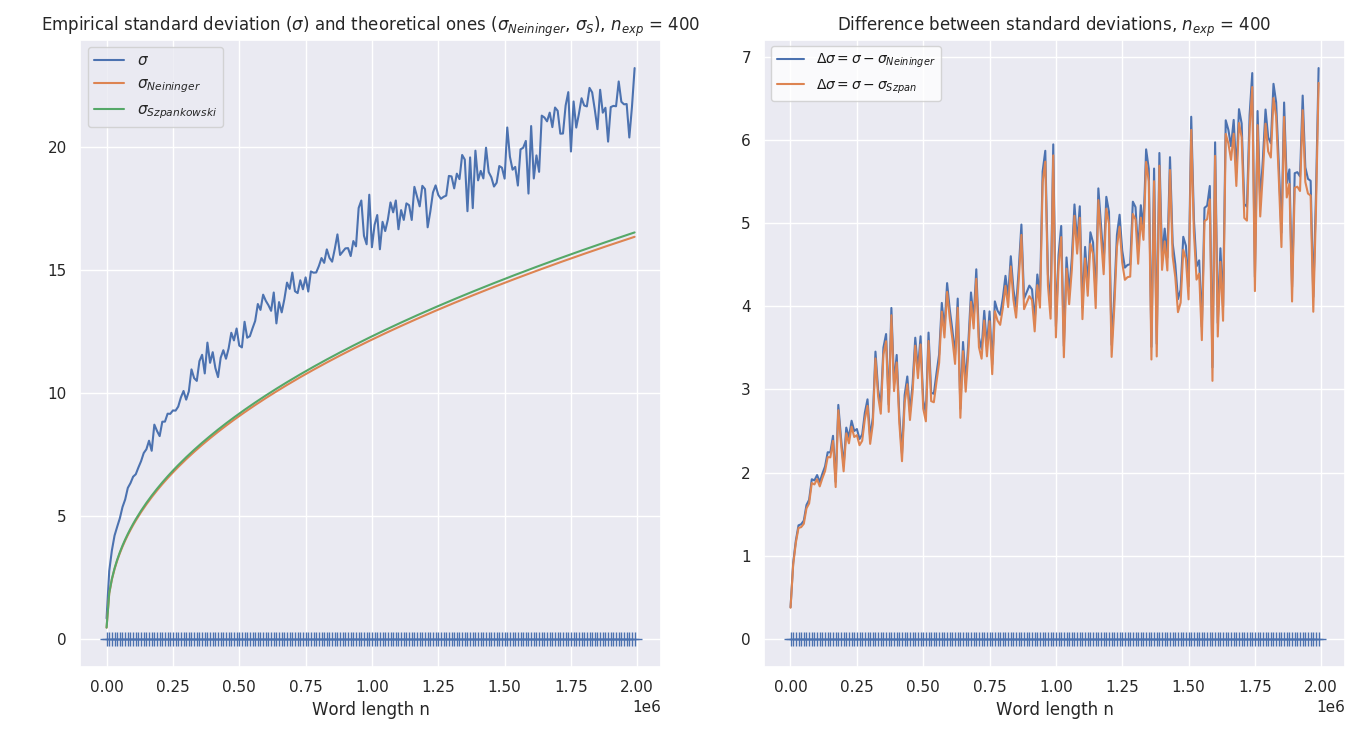
\includegraphics[width = 11cm,
        				    trim = 18.5cm 0 0 0,
        				    	clip=true]{./figs/eig_fig1.png}	
	\end{minipage} 
	}

\pagebreak
Now, for some distributions of very long words that were normalized using 
our theoretical standard deviations, and empirical means. The blue plot is 
a gaussian fit for the simulation results, which also appear as a blue histogram.
The two sets of figures are identical but obtained using different expressions.

\noindent
 	 \begin{minipage}{\textwidth}
        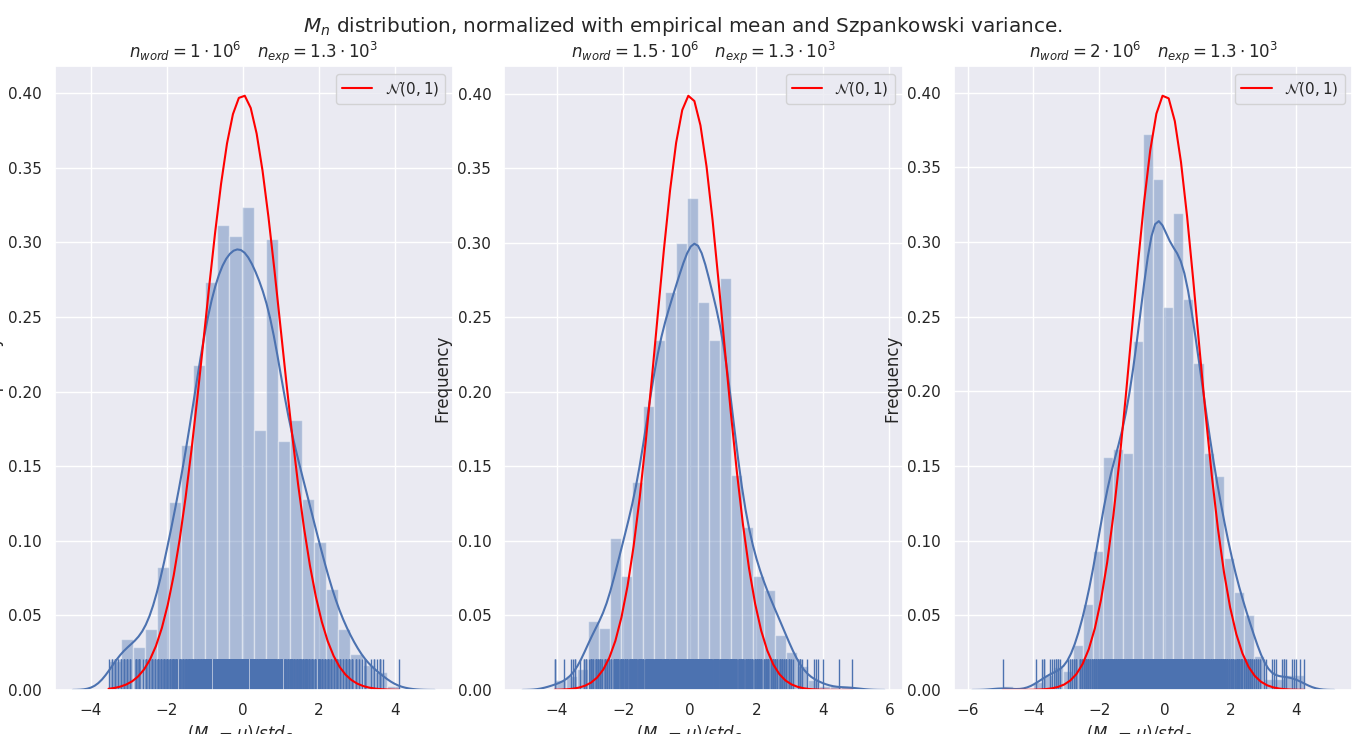
\includegraphics[width = \textwidth,
        				    trim = 0 0.5cm 0 0,
        				    	clip=true]{./figs/eig_fig2.png}	
	\end{minipage} 

\noindent
 	 \begin{minipage}{\textwidth}
        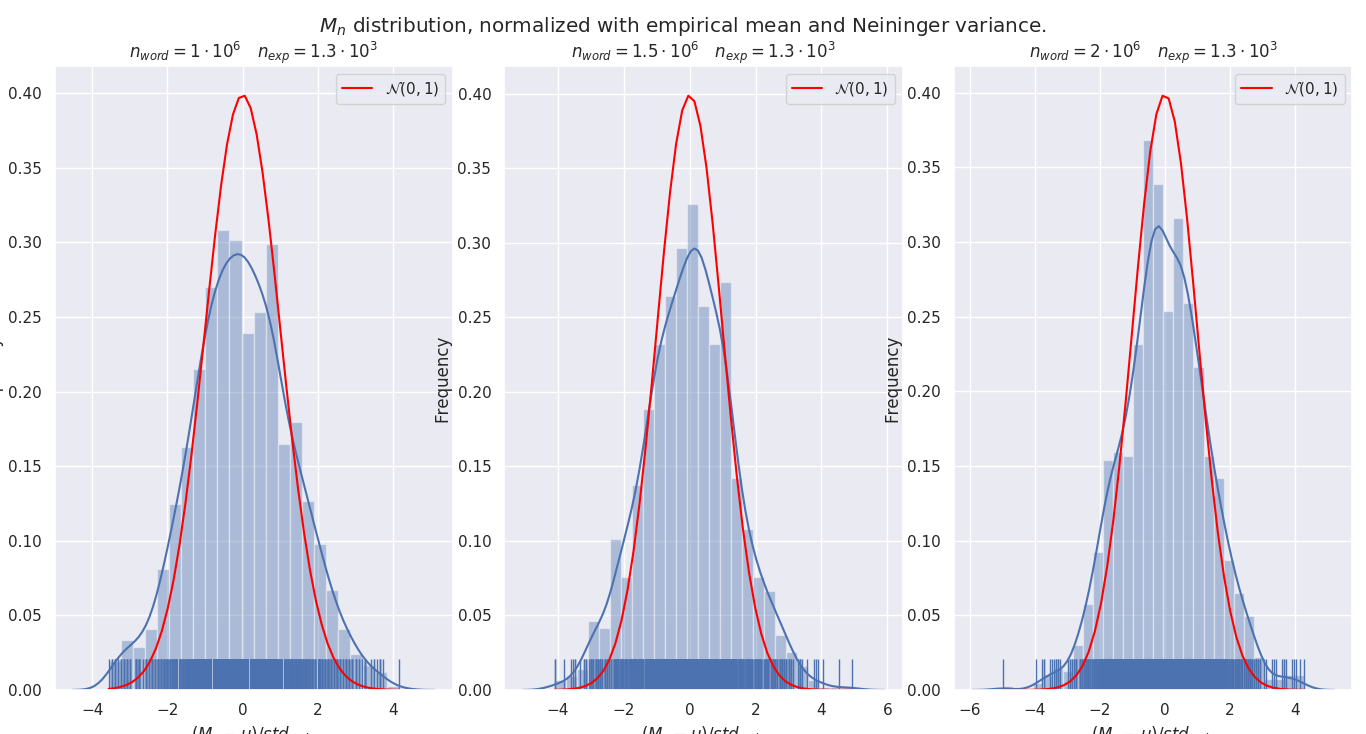
\includegraphics[width = \textwidth,
        				    trim = 0 0.5cm 0 0,
        				    	clip=true]{./figs/eig_fig3.png}	
	\end{minipage} 


\section{Conclusion}
Similar results were obtained for a variety of randomly generated Markov sources,
which seem to indicate that this formula for the variance could be proven theoretically
correct. 

\begin{remarque}
\noindent \textbf{Limits of this work}


The figures suffer from imprecision over the computation of the empirical 
variance : this is due to the difficulties encountered in computing large amounts
of long words (of size over $10^6$). The figure in appendix \ref{app:much_longer} is 
an example of this limitation : with only 100 experiments, the empirical variance 
varies a lot. Possible ideas of improvement might come from parallelization,
rewriting functions in a computationnal language such as Julia, or using/devising a datastructure
specific to the task of building very long words.

Another problem is that the space of random Markov chains (here: stochastic matrices
of size 2) is not sampled thoroughly, therefore this claim might only seem to hold for some
specific Markov chains. Sampling a small number of Markov chains uniformly
according to their entropy might be interesting as a representation of the space,
 because otherwise it would be hard to sample a large number of stochastic matrices
due to the necessity of computing large words for each of them.

Finally, the difference between empirical $V_n$ and our expression seems to be growing
very slowly with $n$. This might be a term that is negligible (\textit{i.e.} of 
order lower than $\tf{n}{\log_2^2(n)}$), or a small detail in the formula of $V_n$. 
For example, the natural base logarithm (in $\tf{n}{\ln^2(n)}$) in the eigenvalue expression works slightly
better than the one in base 2 (in $\tf{n}{\log_2^2(n)}$), with the inverse situation happening for the first 
expression ($\sigma_{\text{Neininger}}$). Anyway, the figures obtained seem to 
indicate that we are close to the exact solution.

\end{remarque}



 
% \noindent First term is
% \centers
%     { $\pi_0 \, p_{0 0} \, \log^2 (p_{0 0}) 
%         + \pi_1 \, p_{1 0} \, \log^2 (p_{1 0}) 
%         + \pi_0 \, p_{0 1} \, \log^2 (p_{0 1}) 
%         + \pi_1 \, p_{1 1} \, \log^2 (p_{1 1})  $}

% \noindent The second is
% \centers
%     { $ - 2 \pac{
%             \dot{\pi}_0(-1) p_{0 0} \log (p_{0 0})    
%             + \dot{\pi}_1(-1) p_{1 0} \log (p_{1 0}) 
%             + \dot{\pi}_0(-1) p_{0 1} \log (p_{0 1})
%             + \dot{\pi}_1(-1) p_{1 1} \log (p_{1 1})
%         }   
%     $}

% \noindent The third is
% \centers{
%     $ - 2 \dot{\lambda}(-1) \pac{
%         \dot{\pi}_0(-1) 
%         + \dot{\pi}_1(-1)
%     }$
% }

% \noindent We 
%         have to compute $\dot{\pi}(-1)$. With 
%             $\pi(s) = (\pi_0(s), \, \pi_1(s))$, and since

% \centers{$\pi(s) P(s) = \lambda(s) \pi(s)$}

% \leftcenters
%     {then we have}
%     {$ \left\{
%         \begin{aligned}
%             {p_{0 0}}^{-s} \pi_0(s) + {p_{0 1}}^{-s} \pi_1(s) &= \lambda(s) \pi_0(s) \\
%             {p_{1 0}}^{-s} \pi_0(s) + {p_{1 1}}^{-s} \pi_1(s) &= \lambda(s) \pi_1(s) \\
%         \end{aligned}
%         \right.
%      $}

% which I'm not sure how to solve formally.
% \noindent
% solving for $\pi_0(s)$ and $\pi_1(s)$, 
% assuming $ p_{0 0} p_{1 1} \neq p_{0 1} p_{1 0} $ :

% \centers{$ \pi_0(s) = \lambda(s) \f{ \overbrace{{p_{1 1}}^{-s} - {p_{0 1}}^{-s}}^{g_0(s)} }
%                                    { \underbrace{{ (p_{0 0} p_{1 1}) }^{-s} 
%                                         - { (p_{0 1} p_{1 0}) }^{-s}}_{\delta(s)} }
%             \qquad 
%             \text{and}
%             \qquad
%        \pi_1(s) = \lambda(s) \f{ \overbrace{{p_{0 0}}^{-s} - {p_{1 0}}^{-s}}^{g_1(s)} }
%                                    { { (p_{0 0} p_{1 1}) }^{-s} 
%                                         - { (p_{0 1} p_{1 0}) }^{-s} }$}


% \leftcenters
%     {hence for $i\in\{0,1\}$}
%     {$ \dot{\pi}_i(s) = \dot{\lambda}(s) \f{g_i(s)}{\delta(s)}
%                         + \lambda(s) \f{{g_i}'(s)\delta(s) - g_i(s)\delta'(s)}
%                                         {\delta^2(s)}$}

% \leftcenters
%     {so}
%     {$ \dot{\pi}_i(-1) = h \f{g_i(-1)}{\delta(-1)}
%                         + \f{{g_i}'(-1) \delta(-1) - g_i(-1) \delta'(-1) }
%                             {\delta^2(-1)} $}

% \begin{egalites}
%     with & \delta(-1) 
%             & p_{0 0} p_{1 1} - p_{0 1} p_{1 0} \\[3mm]
%          &g_0(-1) 
%             & p_{1 1} - p_{0 1} \\[3mm]
%         &{g_0}'(-1)
%             & -\ln (p_{1 1}) p_{1 1} + \ln (p_{0 1}) p_{0 1} \\[3mm]
%         &g_1(-1)
%             & p_{0 0} - p_{1 0} \\[3mm]
%         &{g_1}'(-1) 
%             & -\ln (p_{0 0}) p_{0 0} + \ln (p_{1 0}) p_{1 0} 
% \end{egalites}


% \leftcenters
%     {where}
%     {  $\left\{
%         \begin{minipage}{0.6\textwidth}
%        $ {g_0}'(s) = - \ln(p_{1 1}) {p_{1 1}}^{-s}
%                  + \ln(p_{0 1}) {p_{0 1}}^{-s}$ \\[3mm]
%         $\delta'(s) = - \ln( p_{0 0} p_{1 1}) { (p_{0 0} p_{1 1}) }^{-s}
%                         +  \ln ( p_{0 1} p_{1 0} ) { (p_{0 1} p_{1 0}) }^{-s} $
%         \end{minipage}
%         \right.$ }



% \noindent
% Now taking $s=-1$ and re-arranging in a linear system of unknown $\dot{\pi}_0(-1)$ and $\dot{\pi}_1(-1)$ :
% \centers
%     {$ \left\{
%         \begin{aligned}
%             \dot{\pi}_0(-1) (p_{0 0} - \lambda)
%             + \dot{\pi}_1(-1) p_{0 1}
%                 &= \dot{\lambda}(-1) \pi_0
%                     +   \ln p_{0 0} \cdot p_{0 0} \pi_0
%                     +   \ln p_{0 1} \cdot p_{0 1} \pi_1 \\
%             \dot{\pi}_0(-1) p_{1 0}
%             + \dot{\pi}_1(-1) (p_{1 1} - \lambda)
%                 &= \dot{\lambda}(-1) \pi_1
%                     +  \ln p_{1 0} \cdot p_{1 0} \pi_0 
%                     +  \ln p_{1 1} \cdot p_{1 1} \pi_1
%         \end{aligned}
%         \right.
%      $}

% \noindent since
% $\dot{\lambda}(-1) = h$ and,
% $\lambda(-1) = 1$ :

% \centers
%     {$ \left\{
%         \begin{aligned}
%             \dot{\pi}_0(-1) (p_{0 0} - 1)
%             + \dot{\pi}_1(-1) p_{0 1}
%                 &= h \pi_0
%                     +   \ln p_{0 0} \cdot p_{0 0} \pi_0
%                     +   \ln p_{0 1} \cdot p_{0 1} \pi_1 \\
%             \dot{\pi}_0(-1) p_{1 0}
%             + \dot{\pi}_1(-1) (p_{1 1} - 1)
%                 &= h \pi_1
%                     +  \ln p_{1 0} \cdot p_{1 0} \pi_0 
%                     +  \ln p_{1 1} \cdot p_{1 1} \pi_1
%         \end{aligned}
%         \right.
%      $}

% \begin{egalites}
% which is  &\lambda
%         &\f{ (p_{0 0} + p_{1 1}) 
%            + \sqrt{ (p_{0 0} + p_{1 1})^2 - 4 (p_{0 0} p_{1 1} - p_{1 0} p_{0 1}) }}
%            {2}\\[3mm]
%         &&\f{ (p_{0 0} + p_{1 1}) 
%            + \sqrt{ (p_{0 0} - p_{1 1})^2 + 4 p_{1 0} p_{0 1} }}
%            {2}   
% \end{egalites}






\renewcommand{\subsection}{\oldsubsection}
\renewcommand{\section}{\oldsection}

\section{ Tail symbols analysis}
\renewcommand{\subsection}{\subsubsection}
\renewcommand{\section}{\oldsubsection}
% \section{Tail symbols definition}
% \titre{Tail Symbols}
%%%%%%%%%%%%%%%%%%%%%%%%%%%%%%%%%%%%%%%%%%%%%%%%%%%%%%%%%%%%%%%%%%%%%%%%%%%%%%

% Un aide-m�moire des symboles math�matiques est disponible en ligne:
% http://auteurs.h-k.fr/annales/Doc/aide-memoire/symboles-mathematiques.pdf


\question{The (current ?) definition}
Quoting the paper: 'we call tail symbol the 
symbol that follows the last symbol inserted in the DST'.
What I'm wondering is if the tail symbol is picked from
\begin{itemize}
  \item the same sequence that generated the phrase that was 
        just inserted into the DST
  \item or the beginning of the sequence that follows this phrase ?
\end{itemize}

In the latter case, I'm considering the same example as in 
the paper : the parsing of the eight sequences (these are only their inserted prefixes) :
\centers{$1 \quad 10 \quad 0 \quad 101 \quad 00 \quad 01 \quad 000 \quad 100$}


Is this figure then accurate about the tail symbols ? (I hope not
because this definition seems to contradict other things)
\centers{
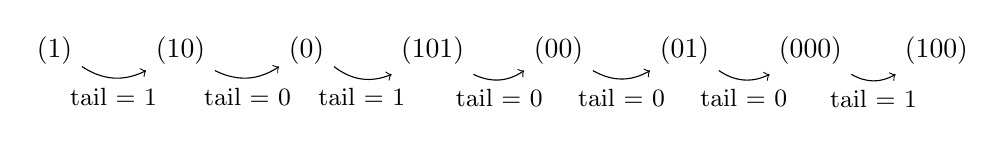
\begin{tikzpicture}[node distance=1.6cm]

% nodes
\node (A) at (0, 0) {(1)};
\node (B) [right of=A] {(10)};
\node (C) [right of=B] {(0)};
\node (D) [right of=C] {(101)};
\node (E) [right of=D] {(00)};
\node (F) [right of=E] {(01)};
\node (G) [right of=F] {(000)};
\node (H) [right of=G] {(100)};

% arrows
\path[->] (A) edge[bend right] node [below] {\small tail = 1} (B);
\path[->] (B) edge[bend right] node [below] {\small tail = 0} (C);
\path[->] (C) edge[bend right] node [below] {\small tail = 1} (D);
\path[->] (D) edge[bend right] node [below] {\small tail = 0} (E);
\path[->] (E) edge[bend right] node [below] {\small tail = 0} (F);
\path[->] (F) edge[bend right] node [below] {\small tail = 0} (G);
\path[->] (G) edge[bend right] node [below] {\small tail = 1} (H);

\end{tikzpicture}}
% Pas de \end{document} ici: voir 'main.tex

Using this definition
  \begin{itemize}
    \item 0 occurs four times as the tail symbol
    \item 1 occurs three times
  \end{itemize}
  
Therefore, in the last paragraph before equation $(1)$, 
${T_8}^{(0)}$ should be $4$ rather than $5$ ? 
And we could now define the tail symbols as \emph{the first
symbol of each sequence except the first one} ? 

But then it seems to clash
with the definition of $T_n = (T_n^a, T_n^b)$, having
$T_n^a$ as the number of times 'a' appears as a tail symbol assuming that
\emph{all} sequences start with symbol 'a'. If \emph{all} means 'all the $n$ sequences'
then the tail symbols definition is absurd because all the tail symbols 
are just 'a' ?

As for the recursion 
\centers{$ T_{n+1}^a = \delta_a + T_{n_a}^a + T_{n_b}^b $}

$\delta_a$ is "equal to 1 when the second symbol of the first sequence is 'a'"
suggests that we should use all the first sequence and not only its prefix 
that is being inserted in the DST ?

Another final problem with this 
definition is that I don't see the probabilistic value of the first
symbol of each independent sequence : I could actually initialize them with any value,
although I'd probably use the stationary distribution to pick that first symbol.

\question{The (right ?) definition}
Therefore I think right now that the definition of the tail symbols
would rather be, since we are in the 
Markov Independent model : if a phrase 
\centers{$ p = w_1 \dots w_n $} is inserted from a sequence 
\centers{$ X = w_1 \dots w_n \,w_{n+1} \dots$}
then the tail symbol of that phrase is $w_{n+1}$. 
Therefore, to define the tail symbols, for example for $n=4$, with the sequences
$X(1) = 00000\dots$, $X(2) = 1010101\dots$, $X(3) = 1001101\dots$ and
$X(4) = 001100111\dots$, which give the parsing 
  \centers{$()(0)(1)(10)(00)$}
we would do, 
with the \textcolor{red}{prefix phrases} in red and the \textcolor{green}{tail symbol} in green :

\begin{egalites}
  & X(1) 
    & {\color{red}{0}} {\color{green}{0}} 00000\dots \\
  &X(2) 
    & {\color{red}{1}} {\color{green}{0}}10101\dots \\
  & X(3) 
    & {\color{red}{10}} {\color{green}{0}} 1101 \dots \\
  & X(4) 
    & {\color{red}{00}} {\color{green}{1}} 100111\dots
\end{egalites}

This means that the tail symbols are not obvious from the DST, 
and this reconciles with the definition of $\delta_a$. If this is the 
correct definition, then the tree of figure 1 is misleading because
we need the sequences to define the tail symbols. (as well as 
the phrase 'in Figure 1 the tail symbol after phrase (10) is "0")







After being done with the variance analysis and 
other tasks such as writing reports on my work 
for P. Jacquet in Paris and my supervisor, I started
working on a new task.

A the heart of it remains the proof central limit theorem for 
LZ'78 on Markov sources - and the results that fall from it.
In the yet unpublished~\cite{jacquet_towards_nodate}, Philippe 
and Wojciech have been working on a new track to proving it.
The difficulty of Markov sources is the dependency between
phrases, which makes it hard to analyze the behavior of 
$M_n$ - the number of such phrases. Their idea is to 
first do the analysis of a simpler variable which is the 
tail symbols count - that we will introduce now.

\section{Markov Independent Model}

Let $M$ a Markov source and $n$ an integer.
The \emph{\bfseries Markov Independent Model} (MI) considers $n$ infinite 
words generated by $M$. The choice of the starting symbol of each sequence
is a parameter of the model. For example, all the sequences
might start with the same letter of the alphabet $c \in \mathcal{A}$.
Or the first symbol could be initialized using the stationary distribution
of the Markov chain related to $M$.

\noindent
This is an example for $n = 4$. These are the sequences :

\[
\begin{array}{cl}
  X(1) &= 00000\dots \\
  X(2) &= 1010101\dots \\
  X(3) &= 1001101\dots \\
  X(4) &= 001100111\dots
\end{array}
\]

\setlength{\parindent}{0pt}
These sequences are used to build a digital search tree
by considering the shortest prefix of each sequence 
that has not appeared yet in the previously considered sequences.
On our example, it yields the parsed word :
  \centers{$()(0)(1)(10)(00)$}
which can be read as the DST :
\centers{
  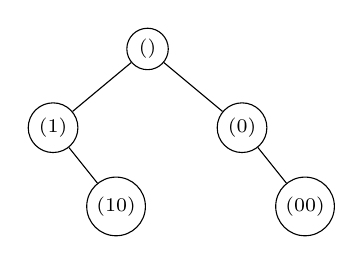
\begin{tikzpicture}[
      level 1/.style={level distance=10mm,sibling distance=24mm},
      level 2/.style={level distance=10mm,sibling distance=16mm},
      level 3/.style={level distance=10mm,sibling distance=16mm},
      font=\scriptsize,inner sep=2pt,every node/.style={draw,circle,minimum size=3ex}]
    ]
    \node {()}
      child {node {(1)}
          child[missing]
          child {node {(10)}}
      }
      child {node {(0)}
          child[missing]
          child {node {(00)}}
      }
          ;
  \end{tikzpicture}
  }

\section{Tail symbols}

\subsection{Definition}

Each of the $n$ sequences possesses a tail
symbol. For each sequence, its \emph{\bfseries tail symbol} is the character that
immediately follows the prefix phrase inserted into the DST.
Therefore the tail symbol is a specific character of this sequence.
If we only have the DST containing the prefix phrases, we cannot
recover the tail symbols.

Visually, with the \textcolor{red}{prefix phrases} in red and the 
\textcolor{green}{tail symbol} in green :

\begin{egalites}
  & X(1) 
    & {\color{red}{0}} {\color{green}{0}} 00000\dots \\
  &X(2) 
    & {\color{red}{1}} {\color{green}{0}}10101\dots \\
  & X(3) 
    & {\color{red}{10}} {\color{green}{0}} 1101 \dots \\
  & X(4) 
    & {\color{red}{00}} {\color{green}{1}} 100111\dots
\end{egalites}

\begin{df}
  Let $c$ be a character from our alphabet $\{ a, b \}$.
  In the case when \emph{all the sequences start with a $c$}, we 
  define \emph{\bfseries $T_n^{\,c}$} the \emph{\bfseries number of times $a$ is a tail symbol in 
  the experiment}.
\end{df}

\begin{rmk}
  \label{rmk:alphaet}
  This is a general definition: for example, in our simulations,
  the alphabet is $\{0, 1\}$ and we only study $T_n^{\,0}$ while
  having all our sequences start with a 0 (initialization step).
\end{rmk}

\subsection{Recurrence relation}

For $n \geq 0$, we have :
    \[ \boxed{ T_{n+1}^{\,c} = \delta_a + 
                            {{\tilde T}_{N_a}}^a
                            + {{\tilde T}_{N_b}}^b } \]

where :
\begin{itemize}
  \item $\delta_a = 
            \begin{cases} 
                1 & \text{if $a$ is the tail symbol of the
                          first sequence}\\
                0 & \text{else} 
              \end{cases}$

  \item $N_a$ is the 
random variable giving \emph{the size of the left subtree 
which contains phrases whose second letter is $a$}

  \item ${{\tilde T}_{N_a}}^a$ is the number of 
times $a$ is a tail symbol for the sequences that were 
used to  build the subtree with phrases having $a$ as second
symbol.

  \item $T_0^c$ for all $c$ by convention.
\end{itemize}

If we take
$\{ N_a = k \}$, then $\{ N_b = n - k \}$, then
the count of the tail symbols on the left tree 
is independent of the one on the right tree :
\textit{i.e.} these quantities are conditionnaly independent.

\section{ Total path length }

In addition to the tail symbols count, introducing the
total path length variable. My task - precisely - was 
to study the asymptotic behavior of the covariance of those 
two variables. I ended up using simulations to gain some precious
insights into the issue, and finally using tools from complex
analysis I found a recurrence relation which would allow 
to find the required asymptotics.

\subsection{ Definition }

Defining \emph{\bfseries $L_n^{\,c}$} as the \emph{total 
path length of the nodes of the DST that was built with
MI model with $n$ sequences starting with letter $c$}.
It is the sum of the lengths of all the prefix phrases.

\subsection{ Recurrence relation }

There is another recursive stochastic relation for 
this quantity, which is, for all $n\geq 0$ :

\[
  \boxed{ 
    L_{n+1}^c = n + 
                        {{\tilde L}_{N_a}}^a + 
                        {{\tilde L}_{N_b}}^b
  }
  \]

with the convention that $L_0^c = 0$ for all $c$.

Same as for the number of tail symbols, this relation 
is found by considering the DST and its two main
subtrees. Except that this time, we count the number 
of times an edge contributes to the path length.
The root with its two nodes contributes as $n$.
The two subtrees contribute respectively for 
${{\tilde L}_{N_a}}^a$ and ${{\tilde L}_{N_b}}^b$.

It is convenient that these two quantities are conditionnaly
independent in the same way as previously seen for the tail symbols.

\section{ Simulating a new model}

The Markov Independent model was different than 
the one I used for my first simulations. At first, 
the asymptotic variable, $n$, represented the length
of the sequence to be parsed with LZ'78. Now, it represented
a number of infinite sequences - or, practically speaking, just 
long enough to be given to LZ'78 in order
for it to extract a prefix a construct its DST. 
It meant that in order to visualize asymptotical behavior,
I'd have to be mindful of performance issue while implementing
it. I partially solved the issue by parallelizing the generation
of sequences using the \emph{\bfseries Multiprocessing} Python
library, and I took a great interest in the newcoming Julia 
language to write an implementation from scratch.

However, the visualizations I obtained - see Figures~\ref{fig:cov} and~\ref{fig:var} 
were already informative,
as we discovered that the behavior of the covariance was 
not as linear as thought, and devised a formal approach to 
estimate it.

\begin{figure}
  \centering
  \includegraphics[width=\textwidth,
            trim = 0 0 0 2cm,
                    clip=true]
    {./figs/cov2.png}
  \caption{Covariance $\Cov(T_n^{\,c}, L_n^{\,c})$ asymptotics\\
          $n_{\text{exp}} = 1546$}
    \label{fig:cov}
  
\end{figure}

\begin{figure}
  \centering
  \includegraphics[width=\textwidth,
                trim = 0 0 0 2cm,
                        clip=true]
    {./figs/var2.png}
  \caption{Dual variance asymptotics\\
                  $n_{\text{exp}} = 1546$}
   \label{fig:var}  
\end{figure}


I then took the path of using the mathematical tools
from combinatorial analytics to solve this issue, and 
left behind the performance issues.


\section{ Poisson tranform differential equation }

This section uses tools from complex analysis and the field 
of combinatorial analytics, which traces back to Philippe
Flajolet. After I spent some time reading Wojciech's and 
Philippe's papers using those tools, I started learning 
them from~\cite{ave}


\subsection{ Covariance recurrence relation }

We want to estimate $\Cov(T_n^{\,c}, L_n^{\,c})$.
Using the previous recurrence relations, we have for all $n\geq 0$ :

\centers{$ \Cov(T_{n+1}^{\,c}, L_{n+1}^c )
           = \Cov( \delta_a + 
                            {{\tilde T}_{N_a}}^a
                            + {{\tilde T}_{N_b}}^b 
                   , n + 
                        {{\tilde L}_{N_a}}^a + 
                        {{\tilde L}_{N_b}}^b) $}

Since the covariance is a bilinear function which is equal
to zero if its two terms are independent or if one is constant,
we can ignore the term $n$ and expand this quantity into six terms :

\vspace{\baselineskip}
$
\begin{array}{rl}
   \Cov(T_{n+1}^{\,c}, L_{n+1}^c) 
    &
            = \Cov( \delta_a, {{\tilde L}_{N_a}}^a )
              + \Cov (\delta_a,  {{\tilde L}_{N_b}}^b)
              + \Cov ( {{\tilde T}_{N_a}}^a,
                         {{\tilde L}_{N_a}}^a ) \\[2mm]
    & \,\,
              + \Cov ( {{\tilde T}_{N_a}}^a, 
                          {{\tilde L}_{N_b}}^b )
              + \Cov ( {{\tilde T}_{N_b}}^b,
                          {{\tilde L}_{N_a}}^a ) 
              + \Cov ( {{\tilde T}_{N_b}}^b, 
                          {{\tilde L}_{N_b}}^b )
\end{array}
$
\vspace{\baselineskip}


Since $\delta_a$ is given by the tail symbol of the first sequence, which
is independent from the rest of the process :
$  \Cov( \delta_a, {{\tilde L}_{N_a}}^a ) = 
       \Cov( \delta_a, {{\tilde L}_{N_b}}^b ) = 0 $

Now, it is not obvious if the pairs $({{\tilde T}_{N_a}}^a, {{\tilde L}_{N_b}}^b)$
and $({{\tilde T}_{N_b}}^b, {{\tilde L}_{N_a}}^a)$ are independent or 
uncorrelated, because the 
random variable $N_a$ is not fixed. However they are conditionnaly independent,
therefore :

\vspace{\baselineskip}

$
\begin{array}{cl}
   \Cov ( {{\tilde T}_{N_a}}^a, 
                          {{\tilde L}_{N_b}}^b )
      & = \Sum{k=0}{n} \Cov ( {{\tilde T}_{N_a}}^a, 
                          {{\tilde L}_{N_b}}^b  \, | \, N_a = k) P(N_a = k) \\[2mm]
      & = \Sum{k=0}{n} \Cov ( {{\tilde T}_{k}}^a, 
                          {{\tilde L}_{n-k}}^b ) P(N_a = k) \\[2mm]
      & = \Sum{k=0}{n} 0 \cdot P(N_a = k) \\[2mm]
      & = 0
\end{array}
$
\vspace{\baselineskip}

Samely, $\Cov ( {{\tilde T}_{N_b}}^b,
                          {{\tilde L}_{N_a}}^a ) = 0$.
Yielding :

  \[ \boxed{ \Cov(T_{n+1}^{\,c}, L_{n+1}^c) = 
          \Cov ( {{\tilde T}_{N_a}}^a,
                         {{\tilde L}_{N_a}}^a )
          + \Cov ( {{\tilde T}_{N_b}}^b, 
                          {{\tilde L}_{N_b}}^b ) } \]


\subsection{ Poisson transform }

Defining 
  \[ \boxed{ C_c(z) 
            = \Sum{n\geq0}{} \Cov(T_n^{\,c}, L_n^{\,c}) 
                            \f{z^n}{n!} \ex{-z} } \]

Computing, with $p = P(a | c)$ and $q = 1-p$ :

\[
\begin{array}{cl}
  \SUM{n\geq 0}{} \Cov ( {{\tilde T}_{N_a}}^a, 
                          {{\tilde L}_{N_a}}^a ) \f{z^n}{n!} \ex{-z} 
      & = \SUM{n\geq 0}{} \Sum{k=0}{n} P(N_a = k) \Cov ( {{\tilde T}_{N_a}}^a, 
                          {{\tilde L}_{N_a}}^a \, | \, N_a = k) \f{z^n}{n!} \ex{-z} \\
      & = \SUM{n\geq 0}{} \Sum{k=0}{n} \binom{n}{k} p^k q^{n-k} 
                          \Cov ( {{\tilde T}_k}^a, 
                          {{\tilde L}_{k}}^a) \f{z^n}{n!} \ex{-z} \\
\end{array}
\]


In this case, $ {{\tilde T}_k}^a $ and $ T_k^a $
as well as $  {{\tilde L}_{k}}^a $
and $  L_k^a$ 
have the same distribution, hence:

\centers{$
\begin{array}{ll}
  \SUM{n\geq 0}{} \Cov ( {{\tilde T}_{N_a}}^a, 
                          {{\tilde L}_{N_a}}^a ) \f{z^n}{n!} \ex{-z} 
      & = \SUM{n\geq 0}{} \Sum{k=0}{n} \binom{n}{k} p^k q^{n-k} 
                          \Cov (  T_k^a, L_k^a)
                           \f{z^n}{n!} \ex{-z} \\
      & = \SUM{n\geq 0}{} \Sum{k=0}{n} 
              \left( \f{(zp)^k}{k!}  \Cov (  T_k^a, L_k^a ) \ex{-zp} \right)
              \left( \f{(zq)^{n-k}}{(n-k)!} \ex{-zq} \right) \\
     &= \underbrace{\left( \SUM{n\geq 0}{} \f{(zp)^n}{n!}  \Cov (  T_n^a, L_n^a ) \ex{-zp} \right)}_{= C_a(zp)}
         \underbrace{\left( \SUM{n\geq 0}{}  \f{(zq)^{n}}{n!} \ex{-zq} \right)}_{= 1} \\
      &= C_a(zp) 
\end{array}
$}

A similar computation gives $ \SUM{n\geq 0}{} \Cov ( {{\tilde T}_{N_b}}^b, 
                          {{\tilde L}_{N_b}}^b ) \f{z^n}{n!} \ex{-z} = C_b(zq) $, 
this time conditionning on $P(N_b = k) = \binom{n}{k} q^k p^{n-k} $.

From what we've seen, when derivating $C_c(z)$ we get :

\[
\begin{array}{cl}
\partial_z C_c(z) 
      &= \SUM{n\geq0}{} \Cov(T_n^c, L_n^c) n \f{z^{n-1}}{n!} \ex{-z} 
         - C_c(z) \\
      &= \SUM{n\geq0}{} \Cov(T_{n+1}^{\,c}, L_{n+1}^c)  \f{z^{n}}{n!} \ex{-z} 
         - C_c(z) \\
      &= \SUM{n\geq0}{} \left[\Cov ( {{\tilde T}_{N_a}}^a,
                         {{\tilde L}_{N_a}}^a )  
          + \Cov ( {{\tilde T}_{N_b}}^b, 
                          {{\tilde L}_{N_b}}^b )\right] \f{z^n}{n!} \ex{-z} 
                - C_c(z) \\
      &= C_a(zp) + C_b(zq) - C_c(z)
\end{array}
\]

Finally the equation for $C_c(z)$ is :

\[
  \boxed{
  \partial_z C_c(z) + C_c(z) 
      = C_a(zp) + C_b(zq)
  }
\]


% Pas de \end{document} ici: voir 'main.tex'

\renewcommand{\subsection}{\oldsubsection}
\renewcommand{\section}{\oldsection}


\section{ Optimal parsing}

\subsection{ LZ77 and LZ78 comparison }

\subsubsection{ Practical uses of LZ77 }

Although it is based on the same approach of identifying 
previously seen phrases - but storing them in a fixed size 
dictionary instead of an evergrowing parse tree like in LZ78 -
the LZ77 algorithm is the most used in practical implementations
of universal compression algorithms.

Let us dive in on a few of the most recent ones :

\begin{itemize}
    \item DivANS
    \item zStandard
    \item 
\end{itemize}

\subsubsection{ }


\renewcommand{\subsection}{\subsubsection}
\renewcommand{\section}{\oldsubsection}
\section{Observations regarding the results and the proof}
\question{Corrections}

\begin{itemize}

\item The formal definition of ${D_n}^{\text{LZ}}$ in $\numero{3}$ is 
      misleading because it contradicts the previous verbal definition.
      For $w$ a word of size $n$, the formula
      \centers{$ \f{1}{M_n(w)} \Sum{j=0}{M_n(w)-1} |{u_j}^{\text{LZ}}|$}
      would rather be the empirical average length of a phrase in the Lempel-Ziv
      parsing of a word ${\barre D_n}^{\text{LZ}}$, whereas
      ${D_n}^{\text{LZ}}$ is used in the rest of the paper as the length
      of a randomly selected phrase. These two aren't equal :
      if we build a Lempel-Ziv DST from a word, then 
      ${D_n}^{\text{LZ}}$ can be seen as the depth of a random node, 
      which is different from the average path length computed 
      on all the nodes. 

\item In \emph{Remark 2}, I think the definition of $v$ and 
      $t$ should rather be 
      $ v = a_{i'} \dots a_{i} $ and
      $ t = a_{i+1} \dots a_n$. 

\item The result $\numero{14}$ should be an equality, and it is one indeed
      because of the flexible parsing algorithm. A proof by contradiction
      can show this. However, since we upperbound $g(j)$ by $\pinf$ in 
      $\numero{23}$ there might be no purpose to using $\numero{14}$ 
      instead of just $\numero{13}$. 
      % Furthermore, an equality is 
      % needed to establish result $\numero{22}$.

\item The proof around \emph{Theorem 1} has several flaws.
      The notation $X$ for a sequence depending on $n$ and not a 
      random variable is misleading. On the other hand, it should appear
      that both $g$ and $j$ are random variables, as the randomness of 
      $j$ is used in the end of the proof.
      I wrote some possible definitions \hyperlink{definitions}{here},
      and applied them to make some computations that seemed otherwise
      incorrect because of their use of randomness outside of a probability
      measure (\hyperlink{computations}{here}).

\item As for the arguments that 
      link $|L_{g(j)-k}|$ to ${D_n}^{\text{LZ}}$, I have
      indicated how I think they could be developped in 
      \hyperlink{critics}{this part.} These arguments
      are the most controversial part right now I think.

\item \emph{Theorem 2} is false as stated: we proved \emph{Theorem 1}
      using a random $j$. The randomness remains, so the quantifier
      'for any $j < M_n$' should be removed. This would be true for 
      \emph{Theorem 1} too.

\item The proof of \emph{Theorem 2} may stop at $\numero{26}$
      since we can directly prove this upperbound goes to $0$.
      This yields a tighter upperbound for \emph{Theorem 2}.
      I detailed this analysis in the 
      \hyperlink{upperbound}{last part of this report.}

\item In that same proof, the step between $\numero{25}$ and 
      $\numero{26}$ relies heavily on a result from $\pac{6}$.
      A bit more context on this result (and why it does apply here)
      would make things clearer.

\item The conclusion claims to use \emph{Cramer's} theorem to link
      \centers{$\underset{ 0 \leq k \leq g_{\scriptscriptstyle W}(J) }{ \max } 
                    \left\{ { L_{g_{\scriptscriptstyle W}(J)-k} - k } \right\}$}
      to ${D_n}^{\text{FLEX}}$, which is a sum of random variables.
      Since \emph{Cramer} applies to independent random variables and the 
      lengths of successive phrases are not independent, something must be missing 
      there.
      
\end{itemize}

\section{Definitions}
\subsection{Definitions}
\newtheorem{Definition}{def}

\question{Notations}

\begin{def}
Let $W$ be the random variable which outputs words of length $n$ 
(of $\Omega_n$) from a memoryless source.
\end{def}

\begin{def}
 Let $J \in \mathbb{N}^{\star}$ be a random
variable which, for every word $w$, uniformly picks the index of
one of its phrases. The joint law of $J$ with $W$ is :

\centers{$ \proba{ W=w, J=j } = 
                    \left\{ \begin{array}{l}
                        \tf{1}{M_n(w)} \quad \textmd{ if } j \leq M_n(w) \\
                        0 \qquad \qquad \textmd{ else }
                    \end{array}
                    \right. $ }
\end{def}

\begin{def}
The function defined as $g$ is a random variable that depends on $W$, therefore
we write it as $g_W$, or, during the event $\{ W=w \}$, $g_w$. 
Samely, we will study the random variable $g_W(J)$, and will
sometimes write $g_w(j)$ when both the events $[W=w]$ and $[J=j]$
occur.


\leftcenters
    {We define the random variable}
    {$B_{J, W}^k = | L_{g_W(J) - k} |$}

\noindent
and we will study the random variable
    {$ \underset{ 0 \leq k \leq g_W(J) }{ \max } 
                    \left\{ { B_{J, W}^k - k } \right\} $}

\noindent
For $J = j$, $W = w$ and $j \leq M_n(w)$, this random variable is the length of 
the $j^{\textmd{th}}$ phrase of the flexible parsing of the word $w$. We have,
accordingly,

\centers{$ D_n^{FLEX} (w) = \f{1}{M_n(w)} \Sum{j=0}{M_n(w)-1} |u_j^{FLEX}|
                          = \f{1}{M_n(w)} \Sum{j=0}{M_n(w)-1}  
                                \underset{ 0 \leq k \leq g_w(j) }{ \max } 
                                \left\{ { B_{j, w}^k - k } \right\} $}
\noindent
Precisely, $D_n^{FLEX}(w)$ is the empirical average of the lengths of the phrases
of the flexible parsing of a word $w$, whereas 
        $\underset{ 0 \leq k \leq g_w(J) }{ \max } 
        \left\{ { B_{J, w}^k - k } \right\} $,
with $J$ a random variable and $w$ fixed,
is the length of a uniformly randomly selected phrase of the flexible parsing
of $w$. 

\leftcenters   
    {Finally, we define}
    {$x_n = \f1{h} \log_2 \pa{ \f{nh}{\log_2(n)} }$}

\leftcenters
    {as well as}
    {$b_n^{\delta} = x_n + (c_3 x_n)^{\delta}$}

\leftcenters
    {and we study}
    {$ \proba{ 
        \underset{ 0 \leq k \leq g_w(J) }{ \max } 
        \left\{ { B_{J, w}^k - k } \right\}
            > b_n^{\delta} } $}

\subsection{Clues in proving the result}

\label{app:critics}
Let $k \in\mathbb{N}$.
Currently, the proof to show this stands on three arguments :

\begin{itemize}
    \item[(1)] The first is that $L_{g_W(J)-k}$ is  
          a random phrase from the Lempel-Ziv parsing of 
          a word of length $N$, where $N \leq g_W(J) \leq n$.
          In the event $\{ N = n' \}$, we consider 
          ${D_{n'}}^{\text{LZ}}$.

    \item[(2)] The second, is that $|L_{g_W(J)-k}|$ can 
          therefore be considered the same as ${D_N}^{\text{LZ}}$
          \textit{i.e} at least equal in law.

    \item[(3)] The third is that, for all $n'\leq n$, 
        ${D_n'}^{\text{LZ}} \leq {D_n}^{\text{LZ}}$.
\end{itemize}
Although they seem generally true,
there are different problems with each of these arguments :

\begin{itemize}
    \item $N$ isn't clearly established, so 
          ${D_N}^{\text{LZ}}$ isn't really known.

    \item If we can identify $N$ and, let's say,
          condition our probability with $\{ N = n' \}$, 
          it is not obvious
          that the choice of a phrase at position ${g_W(J)-k}$
          knowing $\{ N = n' \}$
          is the same as the uniform choice that operates
          when choosing a random phrase from a word of size
          $n'$, in ${D_{n'}}^{\text{LZ}}$.

    \item As for (3), this result is true on average, but 
          not in all cases. Indeed, since ${D_n}^{\text{LZ}}$
          (resp. ${D_n'}^{\text{LZ}}$) is concentrated
          around $x_n$ (resp. $x_n'$), and $x_n'$ < $x_n$
          since $n' < n$, we can show 
          that this result holds with high probability.
          To write the proof, we may condition using
          events of the type

          \centers{$\{ | {D_n}^{\text{LZ}} - x_n | \leq {k_n}^{(1)} v_n \}$}

          \leftcenters
            {and}
            {$\{ | {D_{n'}}^{\text{LZ}} - x_{n'} | \leq {k_n}^{(2)} v_{n'} \} $}
          where 
          \centers{$ v_n = \sqrt{ \log( \tf{nh}{\log(n)} ) } $}
          \noindent
          A sketch of the proof is to
          apply concentration 
          inequalities to these events 
          while picking $({k_n}^{(1)}, {k_n}^{(2)})$ such that 
            \centers{$ {k_n}^{(1)} \, v_n + {k_n}^{(2)} \, v_{n'} < x_n - x_{n'} $}
          \noindent
          and having ${k_n}^{(1)}$ and ${k_n}^{(2)}$ go to $\pinf$ for 
          $n$ going to $\pinf$ in order for the upperbound probability
          to converge to zero. 
\end{itemize}

\subsection{Working with these probabilistic objects}
\hypertarget{computations}{\section{Computations}}
To prove that the definitions I introduced were useful to reason 
and write proof around the subject, I rewrote some computations which
were, in their actual form in the draft, not formally accurate though
understandable.

With these definitions, 
we can do the formal computations at the beginning 
of the proof of \emph{Theorem 1}.

By conditionning on $W$ and $J$, we obtain

\begin{calculs}
        & \proba{ \underset{ 0 \leq k \leq g_W(J) }{ \max } 
        \left\{ { B_{J, W}^k - k } \right\} > {b_n}^{\delta} }
            &=& \Sum{w \in \Omega_n}{} \Sum{j \in \mathbb{N}^{\star}}{} \,
                \proba{ \underset{ 0 \leq k \leq g_W(J) }{ \max } 
        \left\{ { B_{J, W}^k - k } \right\} > {b_n}^{\delta}, W=w, J=j } \\[5mm]
            
            &&=& \Sum{w \in \Omega_n}{} \Sum{j \in \mathbb{N}^{\star}}{} \,
                \proba{ \union{k=0}{g_w(j)} \left\{ B_{w, j}^k > k + {b_n}^{\delta} \right\} 
                            ,W=w, J=j }\\[5mm]
            
            &&\leq&
                \Sum{w \in \Omega_n}{} \Sum{j \in \mathbb{N}^{\star}}{}
                \Sum{k=0}{g_w(j)} 
                \proba{ B_{w, j}^k > k + {b_n}^{\delta}, W=w, J=j } \\[5mm]
            
            &&\leq&
                \Sum{w \in \Omega_n}{} \Sum{j \in \mathbb{N}^{\star}}{}
                \Sum{k=0}{\pinf} \,
                \proba{ B_{w, j}^k > k + {b_n}^{\delta}, W=w, J=j }
                 \\[5mm]

            &&=&
                \Sum{k=0}{\pinf}
                \Sum{w \in \Omega_n}{} \Sum{j \in \mathbb{N}^{\star}}{} \,
                \proba{ B_{w, j}^k > k + {b_n}^{\delta}, W=w, J=j }
                 \\[5mm]

            &&=&
                \Sum{k=0}{\pinf} \,
                \proba{ B_{W, J}^k > k + {b_n}^{\delta} } \\
\end{calculs}




\noindent
For all $k\in\mathbb{N}$, we may now prove that
    \centers{
        $ \proba{ B_{J, W}^k > k + {b_n}^{\delta} } 
            \leq \proba{ {D_n}^{\text{LZ}} > k + {b_n}^{\delta} } $
    }












\section{Proof of an upperbound for the paper}
\hypertarget{upperbound}{}

Finally, while working at the white board with Wojciech, he suggested 
I try a simpler proof for establishing one of the upperbounds in the 
paper goes to 0 as $n$ goes to $\pinf$. This method was, happily, 
a success - and I hope it helps their analysis going forward.
 
 This is a proof that the upperbound 
in $\numero{26}$ goes to 0. Assuming

\centersright{ $ \SUM{k=0}{\pinf} 
            \proba{ D_n^{LZ} (W) > k + b_n^{\,\delta} }
            \leq 
            A \alpha^{ {(c_3 x_n)}^{\delta - \tf12} } 
                \Sum{i=0}{\pinf} \alpha^{ \tf{ i }{ \sqrt{ c_3 x_n } } }
        $}{ \numero{26} }

\noindent We can prove directly that the upperbound term goes to 0 
for $n$ going to $\pinf$,
without resorting to another majoration.
Since $\sqrt{c_3 x_n}$ goes to infinity for $n \rightarrow \pinf$,
we can pick $n$ such that $\sqrt{c_3 x_n} > 1$. Therefore
$\alpha^{\tf{1}{\sqrt{c_3 x_n}}} < 1$ and the geometric sum gives

\centers{ $ \SUM {i=0}{\pinf}
            \alpha^{ \tf{i}{\sqrt{c_3 x_n}} } =
                  \f { 1 } 
                     { 1 - \alpha^{ \tf 1 { \sqrt{ c_3 x_n } } } } $}

\noindent It remains to prove that 
    \centers{$ \underset{n\rightarrow\pinf}{\limt} \,\,\,
                  \f { \alpha^{ {(c_3 x_n)}^{ \delta - \tf12} } } 
                     { 1 - \alpha^{ \tf 1 { \sqrt { c_3 x_n } } }} = 0
            $}

which is done by using L'Hospital's rule.
Define :
\centers
    {$ \fonction
            {f}
            { \Rplusstar }
            { \R }
            { x }
            { \alpha^{ x^{ \delta - \tf12 } } }
      \qquad \text{ and } \qquad
      \fonction
        {g}
        { \Rplusstar }
        { \R }
        { x }
        {  1 - \alpha^{ \f1{ \sqrt{x} } } } $}

\noindent Let $x \in \intoo{0}{\pinf}$. Derivating yields :

\centers{$ f'(x) = \ln \alpha \pa {\delta - \f12}
                    \, x^{\delta - \tf32}
                    \, f(x)
            \qquad \text{ and } \qquad
     g'(x) 
        =  \ln \alpha\,\, \f 1 {2x\sqrt{x}}\, \alpha ^ {\f 1 {\sqrt{x}}} $}

We proceed to show that $\f{f'(x)}{g'(x)}$ goes to 0 as $x$ goes
to $\pinf$. We have

   \centers {
        $ \f{f'(x)}{g'(x)}
             = \f { \pa{\delta - \f12}
                    \, x^{\delta - \tf32}
                    \alpha^{ x^{ \delta - \tf12 } } }
                  { \f{1}{2x\sqrt{x}} 
                        \alpha^{ \f{1}{\sqrt{x}} } }
        = 2 \pa{\delta -\f12} x^{\delta} 
            \cdot \f { \alpha^{x^{\delta-\tf12}}}
                      { \alpha^{ \f{1}{\sqrt{x}} } } $} 

Since $\alpha^{\f{1}{\sqrt{x}}} 
        \underset{x\rightarrow\pinf}{\longrightarrow} 1$, we are left to study 
        $ x^{\delta} \alpha^{x^{\delta-\tf12}}$.

 

\begin{egalites}
 Writing & x^{\delta} \alpha^{x^{\delta-\tf12}}
        & \ex{ \delta \log x + \log \alpha \cdot x^{\delta - \tf12}}
\end{egalites}

and taking the log, since $\delta > \tf12$ and $\log \alpha < 0$ we see that

\centers{$ \delta \log x + \log \alpha \cdot x^{\delta - \tf12} 
            \underset{x\rightarrow\pinf}{\longrightarrow} \minf$}

Therefore $x^{\delta} \alpha^{x^{\delta-\tf12}} \underset{x\rightarrow\pinf}{\rightarrow} 0$,
and given that $f(0) = g(0) = 0$, L'Hospital's rule applies, proving that 
$\f{f(x)}{g(x)} \underset{x\rightarrow\pinf}{\longrightarrow} 0$.






            



\renewcommand{\subsection}{\oldsubsection}
\renewcommand{\section}{\oldsection}

\raggedbottom
\subsection{ Research at Purdue }
During my internship, I worked in the Felix Haas building 
which notably hosts the Center for Science of Information - a research
lab dedicated to information theory problematics. 
Early after my arrival, I started collaborating with some of 
my supervisor's contacts overseas: namely Philippe Jacquet in Paris 
Nokia Labs, and an Italian research team in Palermo -
but I also had the pleasure to discuss, work and spend some time with 
several postdoctoral researchers at Purdue, 
working on Graph Dependency Theory (Abram 
Magner), Information Theory of Communication (Arun Padakandla) and 
other interesting subjects. 
Thanks to them I acquired precious insights 
into the academic environment in the United States. Speaking of which : 
I am sincerely and very thankful to the CSoI and its administration 
for all their help in hosting and organizing my trip. Any trouble 
I could have had was considered and I was able to focus on research 
and writing in very good and peaceful conditions.
Overall, working at Purdue
was a great opportunity which I would recommend to anyone wanting to expand 
their mind about academia and its power to connect people overseas.
It has stirred my interest about doing research abroad - in particular 
in the U.S., and I look forward for another occasion to do so.

\nocite{*}
\bibliographystyle{plain}
\bibliography{bibzot}


\pagebreak


\begin{appendices}

\section{Asymptotics of the mean $E[M_n]$}

	I also tried to normalize $M_n$ using theoretical expressions
	of the mean and variance. For the mean, the first order expression
	
	\centers{$E_n \sim \f{nh}{\log_2(n)}$}
	
	\noindent
	is, under $n\leq 10^6$, not sufficient to center the distribution. I conducted a numerical analysis
	of the difference between this expression and the empirical mean for growing 
	values of $n$. In particular, here is how their difference, in black, compares with
	different approximation functions 
	
	
	  \begin{figure}
		\centering
        \includegraphics[width = 5cm,
        				    trim = 14cm 0 13cm 1.5cm,
								clip=true]{./figs/mean_analysis_2e4_500.png}
		\caption{Difference $\mu - \f{nh}{\log_2(n)}$ and approximation plots.}	
	  \end{figure}
	
	\noindent
	This is not troubling as it was already predicted in the formula:
	
	\centers{$E_n = 	\f{nh}{\log_2(n)} + \mathcal{O} \pa{ \f{n}{\log_2(n)} }$}


\section{Much longer words}
\label{app:much_longer}

\begin{figure}
    \centering
        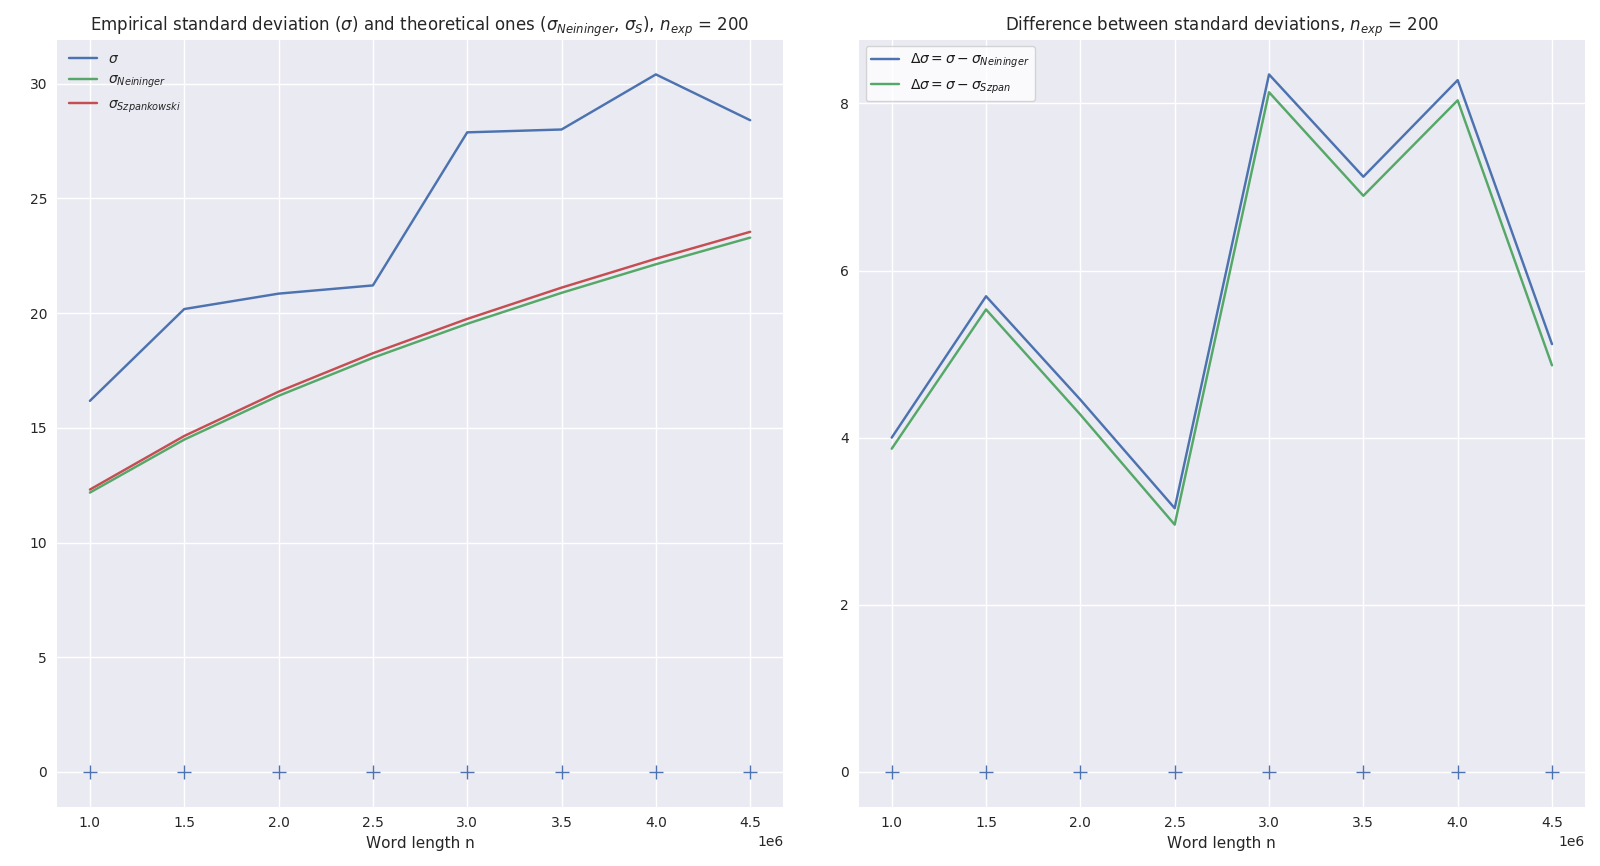
\includegraphics[width = \textwidth,
        				    trim = 0 0 0 0,
                                clip=true]{./figs/eig_fig5.png}	
    \captionsetup{justification=centering}
    \caption{Standard deviations behaviors and difference with empirical\\
            $10^6 \leq n_{\text{word}} \leq 5\cdot10^6, n_{\text{exp}}=200$}
\end{figure}

\noindent
\begin{figure}
    \centering
        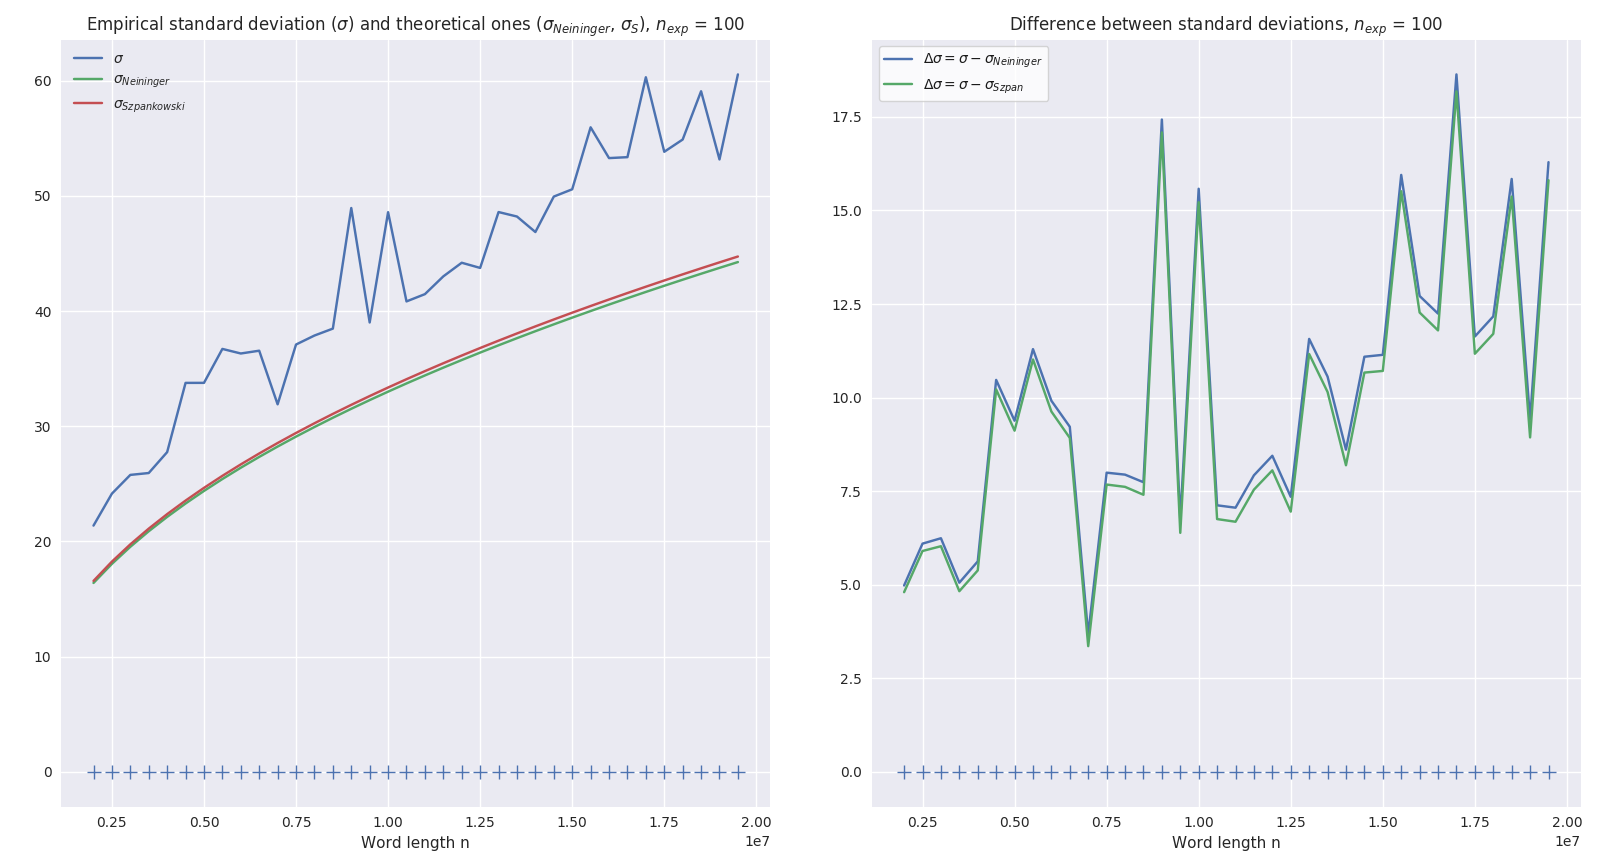
\includegraphics[width = \textwidth,
        				    trim = 0 0 0 0,
                                clip=true]{./figs/eig_fig4.png}	
    \captionsetup{justification=centering}
    \caption{Standard deviations behaviors and difference with empirical\\
    $10^7 \leq n_{\text{word}} \leq 2\cdot10^7, n_{\text{exp}}=100$}
\end{figure}

\pagebreak
\section{Another (more complicated) computation of $\ddot{\lambda}(-1)$}
\label{app:comp_lam1}
This expression gives the sames numerical results as the first one, 
but is more complex to compute for no apparent gain other than having 
yet another similar way of computing $\ddot{\lambda}(-1)$. 
Computing $\delta(s)$, a complex root of 
$\Delta(s)$, writing $\Delta$ as :

\begin{calculs}
    & \Delta 
        &=& \underbrace{p_{0 0}^{-2\Re(s)} \cos(2\ln(p_{0 0})\Im(s))}_{a_0(s)} \\[6mm]
          &&+& \underbrace{p_{1 1}^{-2\Re(s)} \cos(2\ln(p_{1 1})\Im(s))}_{a_1(s)} \\[6mm]
           &&& \underbrace{- 2 (p_{0 0}\,p_{1 1})^{-\Re(s)} \cos(\ln(p_{0 0}\,p_{1 1})\Im(s))}_{a_2(s)} \\[6mm]
           &&+&  \underbrace{4 (p_{0 1}\,p_{1 0})^{-\Re(s)} \cos(\ln(p_{0 1}\,p_{1 0})\Im(s))}_{a_3(s)} \\[6mm]
          &&+& i \Im(\Delta) 
\end{calculs}

where $\Im(\Delta) = b_0(s) + b_1(s) + b_2(s) + b_3(s)$, with each $b_i(s)$ being
the same term as $a_i(s)$ with $\cos$ replaced by $\sin$. Writing

\centers{$\Delta = \alpha(s) + i \beta(s)$}

and searching for $\delta = x(s) + i y(s)$, meaning that

\centers{$ \left\{
                \begin{array}{rl}
                    x^2 - y^2 &= \alpha \\
                    2\, x\, y &= \beta \\
                    x^2 + y^2 &= \sqrt{\alpha^2+\beta^2}
                \end{array}
            \right.
        $}
    

This yields
 
    \centers{$
        \left\{
            \begin{array}{rl}
                     x &= \pm \sqrt{\f{1}{2}(\sqrt{\alpha^2+\beta^2}+\alpha)} \\
                     y &= \pm \sqrt{\f{1}{2}(\sqrt{\alpha^2+\beta^2}-\alpha)} 
            \end{array}
        \right. 
            $}

and since $2xy = \beta$, there is $\epsilon \in \{-1,1\}$ such that
             \centers{$ \delta = \pm (x + \ir \epsilon y) $}

\leftcenters    
    {so}
    {$\lambda(s) = \f{ \poo + \pii \pm (x + \ir \epsilon y)}{2}$}

\leftcenters
    {\text{i.e.}}
    {$\ddot{{\lambda}}(-1) = \f{ p_{0 0} \ln^2(p_{0 0})
                                    + p_{1 1} \ln^2(p_{1 1})
                                    \pm (\ddot{{x}}(-1) + \ir \epsilon \ddot{{y}}(-1))}
                                  {2} $}
where we'll have to find what is $\epsilon$ and which sign to pick.

But first, computing the derivatives of $x(s) = \sqrt{f(s)} $:
    \centers{$\dot{x}(s) = \f{f'(s)}{2x(s)}$}
    \leftcenters
        {and}
        {$\ddot{{x}}(s) = \f{ f''(s) x(s) - f'(s) \cdot \f{f'(s)}{2x(s)} }
                                   { 2 x^2(s) } $}

and then computing $f(s)$ :

    \centers{$ f(s) = \f12 (\sqrt{\alpha^2+\beta^2} + \alpha) $}
    \centers{$ f'(s) = \f12 \left[ \f{ \overbrace{ \dot{\alpha}\alpha + \dot{\beta}\beta }^{ \gamma(s) } }
                                     { \underbrace{\sqrt{\alpha^2 + \beta^2}}_{\kappa(s)} }
                                    + \dot{\alpha} \right] $}

    \leftcenters{with}{$ \dot{\alpha} = \dot{a_0} + \dot{a_1} + \dot{a_2} + \dot{a_3} $}

{As for $f''(s)$, it is}
\centers
    {$ f''(s) = \f12 \left[ 
                        \f{ \dot{\gamma}(s) \kappa(s) - \gamma(s) \dot{\kappa}(s) }
                          {\kappa^2(s)} 
                        + \ddot{{\alpha}}(s) 
                    \right] $}

\leftcenters
    {with}
    {$\dot{\gamma}(s) = \ddot{{\alpha}} \alpha + {\dot{\alpha}}^2 + \ddot{{\beta}}\beta + {\dot{\beta}}^2$}

\centers
    {$ \dot{\kappa}(s) = \f{2 \alpha \dot{\alpha} + 2 \beta \dot{\beta}}
                           {2\sqrt{\alpha^2+\beta^2}}$}


Derivating according to $s$ amounts to derivating according to $\Re(s)$, so in $s=-1$ :

    \centers{$ \dot{\alpha}(-1) = -2\ln p_{0 0} a_0(-1)
                              -2\ln p_{1 1} a_1(-1)
                              -\ln q_0 a_2(-1)
                              -\ln q_1 a_3(-1) $}
and
\centers
    {$ \ddot{\alpha}(-1) = 4\ln^2 p_{0 0} a_0(-1)
                             + 4\ln^2 p_{1 1} a_1(-1)
                              +\ln^2 q_0 a_2(-1)
                              +\ln^2 q_1 a_3(-1) $}

At this point we have fully determined $\ddot{{x}}(s)$, and we realize two things:

\begin{enumerate}
    \item In $s=-1$, since $Im(-1) =0$ and because of the sinus function,
          all the $\beta$ terms, including derivatives, are equal to 0.
          This will simplify the expression for $\ddot{{x}}(-1)$. \\

    \item Furthermore, it also means that $\ddot{{y}}(-1) = 0$,
          so
          \encadre{ $\ddot{{\lambda}}(-1) = \f{ p_{0 0} \ln^2(p_{0 0})
                                    + p_{1 1} \ln^2(p_{1 1})
                                    + \ddot{{x}}(-1) }
                                  {2} $ }
          where the $+$ comes from the fact that $\lambda(s)$ is 
          the highest eigenvalue (and $\ddot{{x}}(-1) > 0$, so by
          continuity the expression around $s=-1$ retained the same sign)
\end{enumerate}

The final expression of $\ddot{{\lambda}}$ (as well as $\dot{\lambda}(-1))$)
can be fully expressed with $\alpha(-1), \dot{\alpha}(-1)$ and $\ddot{{\alpha}}(-1)$.
I empirically verified that $\dot{\lambda}(-1) = h$, and the final result is the same
as with the first method of computation.


% \pagebreak
% \section{Code for computing $\ddot{lambda}(-1)$}
% \label{app:comp_lam2}
% \lstinputlisting[firstline=156,lastline=206]{../src/eigenvalues.py}



\end{appendices}

\end{document}
